% 专业硕士学位论文模板
\documentclass[type = master, class = professional]{whu-thesis}

% 论文信息设置
\whusetup{
  info = {
    title      = {基于平衡损失与多尺度局部适配器的MedSAM腹部多器官分割方法研究}, % 中文标题，可使用 \\ 手动换行
    title*     = {Research on MedSAM Abdominal Multi-Organ Segmentation with Balanced Loss and Multi-Scale Local Adapter}, % 英文标题
    department  = {计算机学院},
    department* = {School of Computer Science},
    author     = {XXX},
    author*    = {XXX},
    student-id = {XXXXXXXXXX},
    supervisor  = {XXX},
    supervisor* = {XXX},
    academic-title  = {教授}, % 导师职称
    academic-title* = {Professor},
    % supervisor-outer = {校外导师}, % 专业学位可能需要校外导师
    % academic-title-outer = {高级工程师},
    major   = {软件工程},
    major*  = {Software Engineering},
    research-area  = {医学图像分割},
    research-area* = {Medical Image Segmentation},
    year = 2026,
    month = 2,
    keywords  = {MedSAM, 类别不平衡, 平衡损失, 多尺度适配器, LoRA消融, 医学图像分割}, % 中文关键词
    keywords* = {MedSAM, class imbalance, balanced loss, multi-scale adapter, LoRA ablation, medical image segmentation}, % 英文关键词
  },
  style = {
    % 字体设置
    font = termes, % 西文字体
    math-font = termes, % 数学字体
    cjk-font = fandol, % 中文字体 (Overleaf用fandol, Windows用windows, Mac用mac)
    % 参考文献设置
    bib-backend = bibtex,
    bib-resource = {ref/references.bib}, % 参考文献数据库
  }
}

\begin{document}

% 目录
\tableofcontents

% 正文开始
\mainmatter

% 引入各章节
\chapter{绪论}

\section{研究背景与意义}

医学图像分割是计算机辅助诊断、术前规划与放疗靶区勾画中的关键基础能力\cite{litjens2017survey}。高质量的分割结果直接影响器官体积估计、病灶边界判读及下游治疗决策。相较于自然图像任务，医学分割长期面临两类共性难题：其一为训练信号分配问题，即目标区域相对背景高度稀疏、困难像素数量有限，致使模型训练易被大量简单像素主导；其二为局部结构表征问题，即边界模糊、低对比、细长或小体积结构往往决定临床可用性，但在以全局建模为主的网络中难以获得充分刻画\cite{hesamian2019survey}。

深度学习的发展持续推动医学分割方法的演进。从全卷积网络（FCN）\cite{long2015fcn}、U-Net\cite{ronneberger2015unet}到 nnU-Net\cite{isensee2021nnunet}，再到基于 Transformer 的 TransUNet\cite{chen2021transunet}与 Swin-Unet\cite{cao2022swinunet}，模型的表征能力与适配范围不断提升。近年来，Segment Anything Model（SAM）\cite{kirillov2023segment}提出了统一的提示式分割范式，其后续版本 SAM 2\cite{ravi2024sam2}进一步扩展至视频场景。MedSAM\cite{ma2024medsam}将 SAM 迁移至医学图像领域，显著增强了模型的通用提示分割能力。然而，当 MedSAM 应用于腹部多器官 CT 分割时，仍暴露出两方面关键不足：一是类别不平衡与困难像素学习不足并存，二是 ViT 编码器对局部边界与高频纹理的建模能力相对欠缺。围绕上述问题开展系统优化，兼具理论研究价值与实际工程意义。

从应用层面而言，腹部多器官分割是医学图像分析中最具代表性的复杂场景之一。其难点不仅在于类别数目较多，更在于不同器官在体积尺度、形态规则性、灰度对比度及邻接关系上存在显著差异。例如，肝脏、脾脏等大器官通常具有较稳定的解剖轮廓，而胰腺、食管、十二指肠及肾上腺等器官往往体积较小、边界模糊、形态不规则，更易成为模型误差的主要来源。因此，在该场景中验证方法，既能检验模型的整体分割能力，又能敏感地暴露训练信号设计与局部结构建模方面的不足。

从研究层面而言，视觉基础模型的迁移正在改变医学图像分割的技术路径。一方面，MedSAM 等模型已具备较强的通用表示与提示驱动能力，使研究者无需从零构建任务专用网络；另一方面，基础模型的强大并不意味着下游任务不再需要针对性优化。对于医学分割而言，如何在不破坏预训练表示优势的前提下进一步重构训练信号、补足局部边界表征、提升困难器官的可分性，仍是一个值得深入探讨的问题。本文正是在这一背景下展开研究：并非试图构建一种全新的医学分割框架，而是围绕 MedSAM 在具体任务中的能力边界进行系统性优化。

从论文工作的意义而言，本文的价值主要体现在两个方面。其一，在方法层面，本文分别从损失设计与结构补强两个方向出发，探讨 MedSAM 当前性能瓶颈的主要来源及优先介入方向；其二，在研究组织层面，本文并非将所有尝试简单堆叠为模块集合，而是通过统一实验协议下的逐步筛选，构建起一条由问题定义、路线比较、负向结果排除到最终方案保留的证据链。

\section{国内外研究现状}

\subsection{医学图像分割模型发展}

医学图像分割方法经历了从传统方法到深度学习，再到视觉基础模型迁移的多阶段演进\cite{wang2022medseg_survey}。

在深度学习时代之前，医学图像分割主要依赖于阈值、区域生长、活动轮廓模型等传统方法\cite{litjens2017survey}。这些方法虽然在特定场景下有效，但严重依赖手工特征设计和先验知识，面对复杂解剖结构和多变成像条件时泛化能力不足。

全卷积网络（FCN）\cite{long2015fcn}的提出标志着深度学习在语义分割中的突破。U-Net\cite{ronneberger2015unet}通过编码器—解码器结构和跳跃连接机制，奠定了医学分割的经典范式。此后，研究者围绕多尺度融合、注意力建模和三维体积信息利用等方向持续改进：UNet++\cite{zhou2018unetpp}通过密集跳跃路径缓解语义鸿沟；Attention U-Net\cite{oktay2018attention}引入注意力门控聚焦目标区域；3D U-Net\cite{cicek20163dunet}和 V-Net\cite{milletari2016vnet}进一步将体积上下文和 Dice 优化引入医学分割任务。

在自动化配置方面，nnU-Net\cite{isensee2021nnunet}通过预处理、网络拓扑和后处理的自适应配置成为医学分割的强基线。在多尺度建模方面，PSPNet\cite{zhao2017pspnet}、DeepLabV3\cite{chen2017deeplabv3}、DeepLabV3+\cite{chen2018deeplabv3plus}和 DenseNet\cite{huang2017densenet}等工作也为密集预测任务提供了重要技术积累。

随着 Transformer 架构进入视觉领域，医学分割进入新的阶段。代表性工作包括 TransUNet\cite{chen2021transunet}、SETR\cite{zheng2021setr}、Swin-Unet\cite{cao2022swinunet}、SegFormer\cite{xie2021segformer}和 UNETR\cite{hatamizadeh2022unetr}，这些方法共同验证了全局自注意力对长距离依赖建模的优势。此后，SAM\cite{kirillov2023segment}和 MedSAM\cite{ma2024medsam}推动了提示式分割在医学场景中的应用。SAM 2\cite{ravi2024sam2}进一步将分割能力扩展至视频和时序场景，但其医学领域适配仍处于早期探索阶段，目前已有的 SAM 2 医学适配工作主要集中在视频超声和内镜序列等时序场景上\cite{zhu2024medsam2}，尚未形成针对静态 CT 切片的成熟方案。围绕医学任务适配，SAMed\cite{zhang2024samed}、Medical SAM Adapter\cite{wu2023medsamadapter}、SAM-Adapter\cite{chen2023sam_survey_med}、SAM-Med2D\cite{cheng2023sammed2d}和 SAM-Med3D\cite{wang2023sammed3d}等工作进一步探索了基础模型的高效适配方式。已有研究普遍表明：基础模型迁移为医学分割提供了新起点，但任务特异性的损失设计与局部结构补强仍然必要\cite{mazurowski2023sam_survey}。

总体而言，医学图像分割模型的发展并非简单的新旧替代，而更体现为优化重心的持续迁移：早期研究主要解决目标区域的基本定位问题，随后转向多尺度结构与长距离依赖的稳健学习，而在基础模型出现后，研究重点进一步转变为在已有强初始化之上补足任务特异性短板。本文选择以 MedSAM 为基座而非从零设计独立网络，正是基于当前研究价值更集中于后一问题的判断。

\subsection{不平衡学习方法}

类别不平衡是医学图像分割中的长期核心问题\cite{litjens2017survey}。在腹部多器官分割中，背景像素通常占据绝大多数，而小器官和边界区域的有效监督信号相对稀缺。

针对类别间不平衡，Class-Balanced Loss\cite{cui2019classbalanced}通过有效样本数建模多数类信息冗余，给出了系统化的类别重加权方法。针对困难样本学习，OHEM\cite{shrivastava2016ohem}提出在线困难样本挖掘策略，Focal Loss\cite{lin2017focal}通过连续调制因子降低易样本权重，GHM\cite{li2019ghm}则从梯度密度角度重新审视样本加权问题。

在损失函数设计方面，Dice Loss\cite{milletari2016vnet}因其对不平衡数据的天然鲁棒性而被广泛使用。Tversky Loss\cite{salehi2017tversky}通过调节假阳性与假阴性权重提供更灵活的平衡机制，Boundary Loss\cite{kervadec2019boundary}则从距离度量角度直接优化边界质量，Active Boundary Loss\cite{wang2022activeboundaryloss}进一步通过动态聚焦边界区域提高边界预测精度。Lov\'{a}sz-Softmax\cite{berman2018lovasz}进一步提供了面向重叠指标优化的代理形式。Unified Focal Loss\cite{yeung2022unified}则尝试从统一建模角度整合不平衡学习策略。总体来看，现有方法大多从“重叠度优化”或“连续调制”角度缓解不平衡，但对类别间重平衡与类别内困难像素加权的联合、可解释建模仍有空间。本文第3章正是在这一问题上，对 MedSAM 的训练信号进行任务驱动的重构。

进一步看，现有不平衡学习方法虽然提供了丰富的技术工具，但其设计出发点往往并非完全针对提示式医学分割场景。一方面，许多方法默认在多类别语义分割或检测框架中使用，其多数类与少数类的划分更多基于类别频次；另一方面，本文任务是在 box prompt 约束下进行二值目标恢复，真正影响性能的因素不仅包括前景与背景的数量差异，还包括同一目标内部困难像素与易分像素之间的梯度竞争。因此，本文的目标并非简单引入某种更强的通用不平衡损失，而是将当前任务中最关键的双层失衡予以显式建模。

\subsection{参数高效微调与局部适配研究}

随着视觉基础模型参数规模持续增长，全参数微调的成本问题日益突出。参数高效微调（Parameter-Efficient Fine-Tuning, PEFT）技术通过冻结大部分预训练参数、仅更新少量任务相关参数来实现任务适配\cite{ding2022peftsurvey}。LoRA\cite{hu2022lora}通过低秩矩阵分解建模权重增量，在自然语言处理任务上取得了显著效果；Visual Prompt Tuning（VPT）\cite{jia2022vpt}、AdaptFormer\cite{chen2022adaptformer}和 Adapter\cite{houlsby2019adapter}等方法也从不同角度验证了轻量级适配的可行性。

然而，在医学图像分割这类强依赖空间重建与边界细节的任务中，单纯冻结主干并不总能维持性能。已有研究指出，ViT 的全局注意力与 CNN 的局部归纳偏置具有较强互补性\cite{dai2021coatnet}。在医学 SAM 适配方向，I-MedSAM\cite{wei2024imedsam}通过高频增强补充边界信息，MA-SAM\cite{chen2024masam}和 Medical SAM Adapter\cite{wu2023medsamadapter}则通过插入卷积适配模块提升空间建模能力。这些工作说明：在医学场景中，合理的结构补强可能比单纯追求参数效率更重要。本文第4章将围绕这一问题，对多条微调与适配路线进行系统比较，并最终收敛到局部适配方案。

这也意味着，对 PEFT 路线的评价标准不应仅停留在新增参数是否最少这一维度。对于需要高质量边界恢复的器官分割任务而言，若参数虽然节省但主干表示无法继续适应具体医学纹理和局部几何特征，则方法的综合收益反而可能受限。正因如此，本文在第4章中并不预设 LoRA 一定优于全参微调，亦不将局部适配器直接视为先验正确方案，而是将其统一纳入比较框架，以突出路线筛选本身的研究意义。

\subsection{视觉基础模型迁移带来的新变化}

视觉基础模型进入医学图像分析后，研究范式出现了明显变化。传统医学分割研究往往从网络结构本身出发，围绕编码器、解码器、跳跃连接或注意力模块进行任务专用设计；而以 SAM、MedSAM 为代表的基础模型路径，则更强调“先获得强通用表征，再进行任务适配”。这意味着研究重点不再只是设计一个从头训练的新网络，而是需要回答另一个问题：对于已经具备较强初始化能力的基础模型，下游性能瓶颈究竟还主要来自哪里。

这一变化带来了两个直接影响。其一，传统方法中许多从零建模的问题在基础模型场景下被部分弱化。例如，MedSAM 已能在较大范围内提供可用的分割初始化，因此简单重复构造新的主干网络未必能带来显著收益。其二，新的问题开始凸显，即如何在保留基础模型已有优势的同时，对医学任务的局部困难区域进行低破坏性补强。本文第3章与第4章的两条主线本质上均建立在这一认识之上：第3章回答基础模型在当前任务中尚缺何种训练信号，第4章回答在训练信号重构后尚缺何种局部表征。

因此，本文并非将基础模型视为需要被完全替换的对象，而更倾向于将其视为一个强基座：它已解决了诸多底层表征问题，但在特定任务中仍保留了若干可被继续优化的薄弱环节。围绕这些薄弱环节开展针对性改进，相较于从零设计复杂框架，更符合当前基础模型时代医学图像分割研究的现实路径。

本文不试图将结论直接外推为通用医学分割方法，而是以腹部多器官 CT 为统一验证场景，聚焦 MedSAM 在该类任务中的两个关键问题：

\begin{enumerate}
  \item \textbf{训练信号分配不足}：在 box prompt 驱动的二值分割范式下，前景像素相对背景高度稀疏，边界与低对比区域中的困难像素又占比较低，常规损失容易被大量简单像素主导。
  \item \textbf{局部边界表征不足}：ViT 编码器更擅长建模全局语义关系，但对边界、高频纹理和细粒度局部结构的响应相对不足，限制了复杂器官边界的进一步提升。
\end{enumerate}

围绕这两个问题，本文将研究目标定位为：以 MedSAM 为基座，构建一条”问题发现—针对性修正—逐步筛选—最终验证”的优化链。具体而言，先通过损失策略重构训练信号，再通过微调/适配路线比较补足局部边界表征，最终形成用于统一展示的最小有效组合。LoRA、Cross-Attention 等未被保留的方案并非作为失败记录，而是作为研究路线收敛的重要证据。

本文通过逐步筛选的方式回答以下基础问题：首先，性能提升究竟主要来自训练信号优化还是结构改动；其次，在训练信号改善之后，剩余误差更接近全局语义不足还是局部边界不足；最后，在可选的多条增强路线中，哪些方案真正与当前任务匹配。

\section{研究目标与技术路线}

\begin{figure}[htbp]
  \centering
  \includegraphics[width=0.85\textwidth]{figures/tech_roadmap.pdf}
  \caption{本文技术路线总览图。图中各方案标注的数值为概要性展示，具体实验结果以正文表格为准。}
  \label{fig:tech_roadmap}
\end{figure}

如图~\ref{fig:tech_roadmap}所示，本文按照”损失策略筛选—适配路线筛选—最终结果验证”的论证顺序展开，而不是简单按实验发生顺序罗列结果。全部实验均在 GT box prompt 条件下进行统一评估，并以 15 个测试病例（10 个 FLARE22 + 5 个 AMOS22）为病例级统计对象，以保证不同方案之间的内部可比性。具体研究步骤如下：

\begin{enumerate}
  \item \textbf{损失策略筛选}：围绕训练信号失衡问题，设计 Balance Loss，并通过组件消融、控制变量验证和补充对照实验，筛选后续统一采用的损失主干。
  \item \textbf{适配路线筛选}：在固定最优损失配置后，比较 Cross-Attention、LoRA 不同秩设置和局部适配器等路线，回答“何种结构增强方式最适合当前任务”。
  \item \textbf{最终结果验证}：仅针对最终保留的里程碑方案，展示总体结果、逐器官表现、边界质量、定性可视化和局限性分析，形成完整的证据闭环。
\end{enumerate}

该技术路线具有明确的问题导向：第一阶段确认训练信号是否为当前性能瓶颈的主要来源，第二阶段判断在训练信号重构后剩余误差是否主要表现为局部边界表征不足。此外，本文保留 BL-$\alpha$1.0 退化、Cross-Attention 回落、冻结主干 LoRA 效果受限等负向结果作为路线收敛的排除性证据，以增强最终方案的说服力。

\section{主要工作与贡献}

围绕上述目标，本文的主要工作与贡献可概括为以下三点：

\begin{enumerate}
  \item \textbf{设计并系统验证了面向训练信号重构的 Balance Loss。} 针对前景/背景失衡和困难像素学习不充分问题，本文设计了将类别间重平衡（Inter-CBL）与类别内困难像素加权（Intra-CBL）联合建模的 Balance Loss，并辅以两阶段训练策略控制引入时机。通过系统的组件消融、超参数敏感性分析和竞争对照实验，确定 BL 为后续统一采用的基础损失配置，为后续结构路线比较提供稳定基座。
  \item \textbf{完成了面向 MedSAM 的多条微调/适配路线的系统比较，并保留局部适配方案。} 本文将 LoRA、Cross-Attention 融合与局部适配器等路线统一纳入比较框架，而非预设某一路线为最优。实验表明，在当前任务和配置下，局部适配方案更能补足边界相关表征，从而形成”Balance Loss + 局部适配”的最终组合。LoRA 和 Cross-Attention 的负向结果作为路线收敛的排除性证据予以保留。
  \item \textbf{通过系统消融与路线对比，建立了当前任务中不同优化策略的适用性判据。} 实验表明，训练信号重构是整体性能提升的首要来源，而局部边界补强在此基础上提供有效补充；Cross-Attention 融合与冻结主干 LoRA 微调等方案的负向结果进一步明确了不同策略在当前任务中的适用边界，使最终方案的选择具有更强的可解释性。
\end{enumerate}

本文的贡献既体现在 Balance Loss 与局部适配器两条方法主线上，也体现在对负向结果的保留与不同策略适用边界的澄清上。后续章节将 BL 与 BL+MSL 作为阶段性里程碑方案重点展开。

\section{论文组织结构}

全文共分六章：

\begin{itemize}
  \item 第1章为绪论，介绍研究背景、相关工作、论文定位与整体技术路线。
  \item 第2章介绍相关理论基础，包括 MedSAM 架构原理、不平衡学习理论、PEFT 技术及局部适配相关理论。
  \item 第3章聚焦 Balance Loss 的配置选择，回答“损失策略如何被筛选出来”。
  \item 第4章聚焦微调与结构增强路线比较，回答“为什么最终选择局部适配而不是其他路线”。
  \item 第5章展示最终保留方案的整体结果、逐器官表现、边界分析、定性可视化与局限性讨论。
  \item 第6章总结全文工作，并讨论后续可进一步扩展的研究方向。
\end{itemize}

\section{本章小结}

本章围绕本文的研究问题、研究动机与论证组织给出了整体说明。本文以 MedSAM 为基座，以腹部多器官 CT 为统一验证场景，围绕训练信号重构与局部边界补强两条主线展开优化，并将实验章节组织为先筛选后展示的研究型叙事结构，为后续章节的展开奠定基础。

\chapter{相关理论与技术基础}

\section{MedSAM 基座模型}

\subsection{SAM 到 MedSAM 的迁移}

SAM（Segment Anything Model）\cite{kirillov2023segment}是一种基于提示的通用分割模型，由 Meta AI 于 2023 年提出。该模型在 SA-1B 数据集（1100 万张图像、10 亿个掩码标注）上训练，建立了"Image Encoder + Prompt Encoder + Mask Decoder"的三段式架构，支持点提示、框提示等多种交互方式。

MedSAM\cite{ma2024medsam}在 SAM 架构基础上进行医学领域迁移，使用超过 150 万对医学图像-掩码标注、涵盖 10 种成像模态和 30 余种肿瘤类型的大规模数据完成领域微调，显著提升了医学场景的适配能力。MedSAM 的微调过程冻结 Prompt Encoder，仅更新 Image Encoder 和 Mask Decoder，采用 Dice Loss 与 Cross-Entropy Loss 的组合作为训练损失函数。其预训练数据中包含了腹部 CT 图像，这为本文的下游任务提供了较好的特征初始化基础（Baseline 在本文统一评估协议下已达到 DSC=0.9407）。MedSAM 发表于 Nature Communications 2024，成为当前医学图像分割领域应用最广泛的基础模型之一。

与传统从零训练的医学分割网络相比，MedSAM 的重要意义在于将提示式分割这一交互范式引入医学图像分析。对于医学场景而言，box、point 等提示不仅是额外的输入形式，更意味着模型无需一次性解决全自动多类别语义理解的全部困难，而可在一定提示约束下聚焦当前目标区域。这种范式尤其适合本文研究的二值器官分割设定：在给定 box prompt 的条件下，模型的核心任务从在整幅图像中识别所有类别转变为在受限区域内准确恢复目标轮廓，从而使训练信号设计与局部边界建模问题更加突出，亦更适合被独立分析。

然而，SAM 向 MedSAM 的迁移并不意味着医学任务中的所有问题均已解决。首先，MedSAM 的预训练虽然提供了较强的通用初始化，但下游腹部多器官 CT 任务仍具有显著的场景特异性：不同器官大小差异悬殊、边界清晰度各异、相邻器官间存在复杂粘连关系。其次，SAM/MedSAM 的核心优势主要体现在可提示、可迁移、可复用的基础模型能力上，而非针对某一特定任务的最优定制。因此，当本文将其用于统一的腹部多器官 CT 评估场景时，更合理的研究问题并非 MedSAM 是否可用，而是在已经可用的前提下，还存在哪些值得继续优化的短板。

在本文任务中，输入为 CT 切片及其 box prompt，输出为二值分割掩码。该设定保留了 MedSAM 的提示式交互优势，同时允许在损失层和特征层进行任务定制。

\subsection{三部分结构解析}

MedSAM 的核心架构由三个模块组成\cite{kirillov2023segment, ma2024medsam}：

\begin{enumerate}
  \item \textbf{Image Encoder}：基于 ViT-Base\cite{dosovitskiy2021vit}，将输入图像（$1024 \times 1024 \times 3$）通过 $16 \times 16$ 的 Patch 嵌入映射到高维语义特征空间，输出 $64 \times 64 \times 256$ 的特征图（16 倍空间下采样）。ViT-Base 包含 12 个 Transformer Block，每个 Block 由多头自注意力层（Multi-Head Self-Attention）和前馈网络（FFN）组成。
  \item \textbf{Prompt Encoder}：将 box/point 等提示映射为位置相关编码，通过位置嵌入将框角点坐标转换为与图像特征对齐的向量表示，约束模型的关注区域。
  \item \textbf{Mask Decoder}：通过轻量级 Transformer 结构融合 Image Embedding 与 Prompt Embedding，经双向交叉注意力（prompt-to-image 和 image-to-prompt）和上采样层生成最终的分割掩码。
\end{enumerate}

在 MedSAM 的标准训练设定中，Prompt Encoder 通常冻结，仅更新 Image Encoder 与 Mask Decoder\cite{ma2024medsam}。图~\ref{fig:medsam_arch}展示了 MedSAM 的三段式架构及数据流向。

从任务分工角度理解，Image Encoder 提供全局语义表征，Prompt Encoder 承担目标区域约束，Mask Decoder 生成最终分割掩码。本文后续改进主要围绕损失层（作用于 Mask Decoder 学习方向）和桥接特征层（作用于 Image Encoder 输出），而 Prompt Encoder 在统一 GT box prompt 前提下不作为主要改动对象。

\begin{figure}[htbp]
  \centering
  \includegraphics[width=0.85\textwidth]{figures/medsam_arch.pdf}
  \caption{MedSAM 三段式架构示意图（Image Encoder + Prompt Encoder + Mask Decoder）}
  \label{fig:medsam_arch}
\end{figure}

\subsection{关键计算流程}

设输入图像为 \(I\)，提示为 \(P\)，可写为：
\begin{equation}
E_I = f_{enc}(I), \quad E_P = f_{prompt}(P), \quad \hat{Y}=f_{dec}(E_I,E_P)
\end{equation}
其中 \(E_I\) 为图像语义特征，\(E_P\) 为提示特征，\(\hat{Y}\) 为预测掩码。本文后续改进主要作用于 \(f_{dec}\) 的特征融合输入（第4章局部适配器）与训练目标函数（第3章 Balance Loss）。

从这一计算流程可以看出，在本文统一采用 GT box prompt 的条件下，模型性能差异主要来自图像特征的表达质量与监督信号的引导方式。本文后续改进围绕这两个方面展开。

\section{类别不平衡理论}

\subsection{有效样本数与长尾重加权}

Class-Balanced Loss\cite{cui2019classbalanced}指出，样本数量并不等价于信息量，提出有效样本数定义：
\begin{equation}
E_n = \frac{1-\beta^n}{1-\beta}
\end{equation}
其中 \(n\) 为样本数，\(\beta \in [0,1)\)。其核心直觉是：每个新样本以概率 $\beta$ 落入已有原型的覆盖范围（即成为冗余样本），信息增益以 $\beta$ 的指数速率递减。当 $\beta \to 0$ 时 $E_n \to 1$（所有样本近乎相同），当 $\beta \to 1$ 时 $E_n \to n$（每个样本完全独特）。当 \(n\) 很大时，\(E_n\) 增长趋缓，反映多数类信息冗余。

对于医学分割像素级任务，背景像素数量常远大于前景像素数量。若不进行再平衡，多数类将持续主导梯度方向，使模型更偏向背景预测。有效样本数理论为"削弱冗余背景影响"提供了数学依据。具体而言，设前景像素数为 $n_f$、背景像素数为 $n_b$（$n_b \gg n_f$），则标准 BCE 损失中两类梯度的总贡献量之比近似为 $n_b : n_f$，多数类的梯度将主导参数更新方向。有效样本数理论给出的再平衡权重为 $w_c = 1/E_{n_c}$，使得每一类对总梯度的贡献不再与原始像素数成正比，而与该类所携带的有效信息量成正比。第3章中 Inter-CBL 的困难背景挖掘可以看作该思想在像素级的一种操作性实现：不是对所有背景像素施加统一降权，而是直接丢弃信息冗余度最高的简单背景像素，仅保留与前景数量对齐的困难背景子集参与梯度计算，从而在控制梯度比例的同时保留最具信息量的负样本。

\subsection{困难样本挖掘}

OHEM（Online Hard Example Mining）\cite{shrivastava2016ohem}通过在每个前向传播中计算所有候选样本的损失值，按损失降序选取 top-$k$ 样本参与反向传播，从而将训练信号集中于当前模型最难正确处理的样本。Focal Loss\cite{lin2017focal}则采用连续调制因子 $-(1-p_t)^\gamma \log(p_t)$ 实现对困难样本的软聚焦，其中 $p_t$ 为模型对真实类别的预测概率，$\gamma$ 控制聚焦强度。当 $\gamma > 0$ 时，高置信度的易分样本（$p_t \to 1$）的调制因子 $(1-p_t)^\gamma \to 0$，其损失贡献被大幅压制；而低置信度的困难样本（$p_t \to 0$）所受压制较小，从而在梯度层面获得相对更高的权重。

两者共同目标是降低易样本对梯度的主导，提升困难样本学习效率。但两种机制在实现方式上存在重要差异：OHEM 采用硬阈值选择（保留或丢弃），Focal Loss 采用连续软调制（按置信度平滑降权）。第3章中 Intra-CBL 的设计介于两者之间——采用基于置信度误差阈值 $\tau$ 的二值分段权重（易/难二分），在保持可解释性的同时避免了 OHEM 完全丢弃易样本信息的风险。第3章实验中 Baseline-Focal 的对照结果将进一步表明，Focal Loss 的连续调制在当前像素级二值分割任务上并未自动转化为更好的训练信号，其原因可能在于 $\gamma$ 参数对所有像素施加统一形式的调制，无法像 Balance Loss 那样针对类别间与类别内分别定制再平衡机制。

\subsection{与本文任务的对应}

本文任务中的困难样本主要集中于器官边界、弱对比区域及形态突变区域。相比通用目标检测场景，医学分割更强调边界质量，因此困难样本加权不仅影响 DSC，也会影响 HD95 与 ASD。

进一步地，本文任务中的“不平衡”并不是单一层面的类别频次问题，而具有更复杂的双层结构。其一，在前景与背景之间，背景像素数量远大于前景，若采用常规等权 BCE 或 Dice+CE 训练，模型更容易通过拟合大量简单背景像素获得较低损失，从而削弱对前景区域的关注；其二，在同一类别内部，器官边界、低对比区域和细长结构等困难像素数量远少于内部均质区域，导致即便模型已经学会大体轮廓，也可能在真正决定临床可用性的局部区域表现不佳。

这一特点决定了本文不能简单照搬自然图像场景下的类别平衡策略。对于医学分割而言，仅从“前景—背景”角度做重加权，往往不足以显著改善边界质量；而若只关注类内困难样本，又可能忽略背景中大量冗余像素对梯度方向的主导作用。因此，第3章中 Balance Loss 的设计并不是单纯把已有损失相加，而是尝试同时回应这两个层面的训练信号失衡问题：Inter-CBL 主要缓解类别间的不均衡，Intra-CBL 主要提升类别内困难像素的学习权重，二者共同构成对当前任务的针对性建模。

\section{损失函数基础}

本节概述本文方法设计涉及的基础损失函数。表~\ref{tab:loss_overview}以统一视角总结各损失的核心公式、优化目标与关键特性，为第3章 Balance Loss 的设计提供理论背景。

\begin{table}[htbp]
  \centering
  \caption{医学分割常用损失函数概览}
  \label{tab:loss_overview}
  \small
  \begin{tabular}{llp{5.5cm}}
    \hline
    损失函数 & 核心公式 & 关键特性 \\
    \hline
    BCE\cite{goodfellow2016deeplearning} & $-\frac{1}{N}\sum[y_i\log p_i+(1{-}y_i)\log(1{-}p_i)]$ & 像素级独立优化，对困难像素无差别对待 \\
    Dice\cite{milletari2016vnet} & $1-\frac{2|Y\cap\hat{Y}|}{|Y|+|\hat{Y}|}$ & 全局重叠度优化，天然对类别不平衡鲁棒，但单像素梯度被全局统计量稀释 \\
    Focal\cite{lin2017focal} & $-\alpha_t(1{-}p_t)^\gamma\log(p_t)$ & 连续调制因子自动降低易样本权重，$\gamma$ 控制聚焦强度 \\
    Tversky\cite{salehi2017tversky} & $1-\frac{|Y\cap\hat{Y}|}{|Y\cap\hat{Y}|+\alpha_{tv}|FN|+\beta_{tv}|FP|}$ & 可调 FN/FP 权重，灵活控制召回率-精确率平衡 \\
    Boundary\cite{kervadec2019boundary} & $\int_\Omega \phi_G(\mathbf{q})s_\theta(\mathbf{q})d\mathbf{q}$ & 基于符号距离函数直接优化边界距离 \\
    Active Boundary\cite{wang2022activeboundaryloss} & 动态聚焦边界区域 & 在训练中逐步聚焦边界附近像素，提高边界预测精度 \\
    \hline
  \end{tabular}
\end{table}

其中，BCE 与 Dice 是本文的核心基础组件。两者在梯度性质上具有互补性：Dice Loss 的梯度包含形如 $\frac{2(y_i|\hat{Y}|-|Y\cap\hat{Y}|)}{(|Y|+|\hat{Y}|)^2}$ 的全局归一化项，使其对类别不平衡天然鲁棒，但单个困难像素的梯度贡献会被集合统计量稀释；BCE 则逐像素独立计算梯度，对困难像素的纠正更为直接。这一互补性是 MedSAM 原始训练及本文损失设计中联合使用两者的理论基础。Focal Loss 在后续实验中作为不平衡损失的对照基线进行评估（第3章 Baseline-Focal 配置）。

\section{参数高效微调理论}

\subsection{LoRA 低秩适配}
\label{sec:lora_theory}

随着大模型参数规模急剧增长，参数高效微调（PEFT）成为迁移学习的重要范式\cite{ding2022peftsurvey}。LoRA（Low-Rank Adaptation）\cite{hu2022lora}是其中最具代表性的方法，其核心思想是对预训练权重矩阵的增量施加低秩约束：

\begin{equation}
W = W_0 + \Delta W = W_0 + BA, \quad B \in \mathbb{R}^{d \times r}, \, A \in \mathbb{R}^{r \times k}, \, r \ll \min(d,k)
\end{equation}

训练过程中冻结原始权重 $W_0$，仅更新低秩矩阵 $A$ 和 $B$，可将可训练参数量减少数个数量级。LoRA 在 NLP 领域应用广泛，但在密集预测的医学图像分割任务上，冻结视觉编码器是否可行仍存在争议——这正是本文第4章通过 LoRA 路线比较重点讨论的问题。

\subsection{Adapter 架构}

Adapter\cite{houlsby2019adapter}是另一类参数高效微调策略，通过在预训练模型的层间插入小型瓶颈模块来实现任务适配。与 LoRA 的区别在于：Adapter 引入了额外的网络结构（而非修改现有权重矩阵），因此可以灵活选择在模型的不同位置注入不同类型的归纳偏置。

对于本文任务而言，LoRA 与 Adapter 的关键差异在于：LoRA 以低秩增量修正已有表示，而 Adapter 允许在特定层位注入局部卷积、多尺度分支等任务相关归纳偏置。对于需要精细边界重建的医学分割任务，后者的结构可定制性往往更为重要。

\section{卷积归纳偏置与 ViT 互补性}

\subsection{ViT 的全局建模优势与局部缺陷}

Vision Transformer\cite{dosovitskiy2021vit}通过全局自注意力机制建模图像中任意两个 Patch 之间的关系，具有强大的远距离依赖捕获能力。然而，自注意力对所有空间位置一视同仁，缺乏卷积网络固有的局部平移不变性和空间层次性\cite{dai2021coatnet}。在医学图像中，器官边缘通常表现为高频局部特征，ViT 的全局建模倾向会"平滑"掉这些关键信息。

对于腹部多器官 CT 场景而言，这一缺陷尤其值得关注。大器官的分割更多依赖整体位置与形状先验，而小器官、细长器官和相邻粘连区域则更依赖局部纹理变化与细粒度边界线索。若缺少适当的局部归纳偏置补充，模型在这些高频细节区域容易产生边界过平滑或局部欠分割等现象。

\subsection{CNN 的局部归纳偏置}

卷积神经网络通过有限大小的卷积核具备局部连接和权值共享特性，对局部纹理和边缘模式具有较强归纳偏置\cite{he2016resnet}。深度可分离卷积\cite{howard2017mobilenets}进一步将标准卷积分解为逐通道的空间卷积和逐点的通道混合，在大幅降低参数量的同时保留了空间局部特征提取能力。膨胀卷积（Atrous Convolution）\cite{yu2016dilated}则通过在卷积核元素之间插入空洞来扩展感受野，能够在不增加参数量的情况下实现多尺度特征提取\cite{chen2018deeplabv3plus}。

\subsection{混合架构的理论基础}

近年来，CoAtNet\cite{dai2021coatnet}等研究表明，将卷积的局部归纳偏置与 Transformer 的全局注意力相结合，能够在各种数据规模下获得比纯 ViT 或纯 CNN 更优的性能。此外，CvT（Convolutional vision Transformers）\cite{wu2021cvt}从 Token 嵌入角度出发，在每个 Transformer 阶段使用卷积投影替代线性投影来生成 Query、Key、Value，从而在不改变整体 Transformer 框架的前提下引入局部空间结构信息；LocalViT\cite{li2021localvit} 则在 FFN 层中嵌入深度可分离卷积，使每个 Transformer Block 在前馈过程中同时完成局部特征增强与通道混合，以极小的参数开销弥补 ViT 对局部纹理的感知不足。这些工作从不同的架构层级（Token 嵌入层、注意力投影层、FFN 层）验证了同一结论：在 Transformer 中适当注入卷积归纳偏置，能够系统性地提升模型对局部高频特征的建模能力。这一思想为在 ViT 编码器的输出特征上叠加卷积层提供了理论支撑，使模型可同时具备全局语义理解和局部边缘捕获能力。

该理论表明，局部归纳偏置并不一定需要在模型前端大规模重写主干，也可以在已具备强全局语义表示的桥接特征层上以较小代价补入，从而兼顾预训练优势与局部边界建模需求。

\subsection{卷积参数在桥接特征分辨率下的有效性分析}

在 MedSAM 中，Image Encoder 将 $1024 \times 1024$ 的输入图像以 $16\times$ 下采样映射为 $64 \times 64 \times 256$ 的特征图。在此分辨率下，特征图上的一个像素对应原始图像中 $16 \times 16$ 的空间区域。标准 $3\times3$ 卷积核（$d{=}1$）在特征图上的感受野为 $3 \times 3$，映射回原始图像为 $48 \times 48$ 像素，约覆盖单个小器官（如肾上腺）在典型切片上占据区域的 1/3--1/2。膨胀率 $d{=}2$ 的 $3\times3$ 卷积核的等效感受野为 $5 \times 5$（特征图坐标），映射回原始图像为 $80 \times 80$ 像素，可覆盖中等器官的邻域或小器官的完整轮廓范围。

因此，在 $64 \times 64$ 桥接特征图上使用 $d{=}1$ 和 $d{=}2$ 的双路径卷积，分别提供了"边界精细响应"和"局部上下文感知"两个尺度的归纳偏置。这一分析说明，第4章中 MSL-Adapter 选择 $3\times3$ 标准卷积与 $3\times3$ 膨胀卷积的组合并非任意搭配，而是基于桥接特征图的空间分辨率与目标器官的典型尺度之间的匹配关系。

\section{注意力机制与交叉注意力融合}

\subsection{自注意力机制}

Transformer 的核心计算组件是自注意力（Self-Attention）\cite{vaswani2017attention}。给定输入序列，通过线性投影得到查询（Query）、键（Key）、值（Value）三组向量，注意力输出为各位置值向量的加权和，权重由查询与键的缩放点积经 softmax 归一化得到。多头自注意力（Multi-Head Self-Attention, MHSA）将特征空间拆分为多个子空间独立计算注意力后拼接，使模型能够同时关注不同位置的不同语义子空间。

在 MedSAM 的 Image Encoder（ViT-Base）中，输入图像被划分为 $64 \times 64 = 4096$ 个 Patch Token，自注意力在所有 Token 之间建立全局交互。这种全局建模能力是 ViT 捕获远距离依赖的核心优势，但其计算复杂度为 $O(N^2)$，且对所有空间位置施加均匀的注意力权重，不具备卷积的局部优先归纳偏置。

\subsection{交叉注意力机制}

交叉注意力（Cross-Attention）是自注意力的推广形式，允许来自不同来源的特征进行信息对齐与融合。与自注意力的区别在于：Query 来自一个序列（查询源），而 Key、Value 来自另一个序列（参考源）。

交叉注意力在 MedSAM 中已有两处典型应用：Mask Decoder 中的 prompt-to-image 注意力（以提示 Token 为 Query，以图像特征为 Key/Value）和 image-to-prompt 注意力（方向相反），两者共同实现提示信息与视觉特征的双向对齐。

\subsection{交叉注意力在少样本分割中的应用}

在少样本分割（Few-Shot Segmentation）领域，交叉注意力被广泛用于建立支持样本（support）与查询样本（query）之间的特征对齐。PANet\cite{wang2019panet}提出的 support-query 原型对齐是典型应用：从支持样本中提取类别原型，通过注意力机制将其与查询图像特征对齐，从而将已有的分割知识迁移到新样本。这一思路的核心假设是：参考样本能够为当前样本提供有价值的类别先验或结构模板。

第4章中的 BL+CA 路线正是受此思想启发：以当前样本的编码器特征为 Query，以同类器官参考样本的特征为 Key/Value，尝试通过跨样本参考信息来补充当前特征的不足。然而，这种策略在与已具备稳定医学迁移初始化的预训练模型结合时需要审慎评估。对于 MedSAM 而言，其 Image Encoder 已在大规模医学数据上建立了较为完善的器官语义表征，此时额外注入的跨样本参考特征可能与原有特征分布不一致，进而破坏预训练表征的稳定性。此外，交叉注意力引入的跨样本依赖还会增加推理阶段的复杂度（需预先编码参考样本），在实际部署中带来额外负担。

因此，若当前误差主要来自局部边界表征不足而非全局语义不充分，继续向桥接层注入跨样本参考信息未必比直接补足局部归纳偏置更具针对性。这一分析性判断将在第4章通过实验加以验证。

\section{评价指标与实验口径}

本文统一采用以下指标评价模型分割性能\cite{taha2015metrics}：
\begin{itemize}
  \item DSC（Dice Similarity Coefficient）：衡量重叠一致性，越高越好；
  \item HD95（95\% Hausdorff Distance）：衡量边界最大偏差的鲁棒版本，越低越好；
  \item ASD（Average Surface Distance）：衡量平均表面距离，越低越好。
\end{itemize}

这三类指标分别对应分割性能的不同维度：DSC 更强调整体区域重叠程度，适合反映模型是否学到了器官的大体轮廓；HD95 对极端边界误差更敏感，能够反映预测掩码在最差局部位置上的偏离情况；ASD 则刻画平均意义下的边界贴合质量，更适合衡量模型在整体轮廓细化上的稳定性。对于本文研究而言，仅报告 DSC 往往不足以揭示方法改进真正发生在哪里，因此第3章至第5章均将三项指标联合使用，以分别观察训练信号重构与局部适配对“整体重叠”和“边界质量”的不同影响。

此外，本文在结果汇报中统一以病例为统计单位，而不直接以切片为单位汇总平均值。这一做法的意义在于：切片数目受器官体积和病例层厚影响较大，若直接做切片级平均，容易使大体积器官或长体积病例在统计上占据更高权重；而病例级统计更能反映方法在实际个体层面的稳定性，也更适合作为后续 Wilcoxon 配对检验的输入。由此，第5章中的统计显著性分析不仅是形式上的补充，也与本文整体实验口径保持一致。

本文统一采用 FLARE22\cite{ma2022flare}与 AMOS22\cite{ji2022amos}数据集各自测试集中的 10 个和 5 个病例作为同口径评估对象，所有实验均在 GT box prompt 条件下进行统一评估。数据来源、评估对象、提示形式与统计粒度的详细设定见第5章。

\section{本章小结}

本章系统梳理了本文方法所依赖的理论与技术基础：MedSAM 架构与计算流程、不平衡学习理论、困难样本挖掘机制、常用损失函数、参数高效微调（LoRA/Adapter）原理、卷积归纳偏置与 ViT 的互补性理论、交叉注意力融合及统一评估口径。上述内容共同构成第3至5章方法设计与实验分析的理论基础。

\chapter{联合平衡损失框架的设计与配置筛选}

本章聚焦于回答一个明确问题：在对 MedSAM 进行后续结构增强之前，何种损失配置最适合作为统一采用的训练主干。与按实验发生顺序罗列结果不同，本章按论证逻辑组织证据：先定义训练信号分配问题，再给出 Balance Loss 的方法设计，随后通过统一比较筛选最终配置，并以补充分析验证该配置的合理性。本章的目标不在于展示实验历程，而在于说明后续章节统一采用 BL 作为损失主干的依据。

\section{问题定义与方法设计}

在 MedSAM 的提示式分割框架下，模型输出本质上是前景/背景二值掩码。医学图像场景中，前景像素通常显著少于背景像素，而边界、低对比和形态复杂区域中的困难像素又只占少数。由此带来的问题并不只是传统意义上的类别不平衡，更表现为训练信号在“类别间”和“类别内”两个层面同时分配不均：一方面，大量简单背景像素会在梯度上压制前景区域的学习；另一方面，即使在同一类别内部，困难像素也容易被大量易分像素淹没。

针对这一问题，本文设计联合平衡损失框架 Balance Loss，将类别间平衡（Inter-CBL）与类别内困难像素加权（Intra-CBL）联合建模，并通过两阶段训练缓解训练初期的噪声干扰。

需要说明的是，本文所提 Balance Loss 与 Cui 等人\cite{cui2019classbalanced}的 Class-Balanced Loss 在名称上存在相似性，但两者的设计目标与技术路线不同。Class-Balanced Loss 基于有效样本数理论对多类别分类任务中的长尾类进行损失重加权，属于单一层面的类别间重平衡策略。本文 Balance Loss 则针对医学分割中像素级监督信号在"类别间"和"类别内"两个层面同时失衡的问题，将 Inter-CBL（困难背景挖掘）与 Intra-CBL（困难像素加权）联合建模，并辅以两阶段训练策略控制引入时机。因此，两者虽然共享"平衡"的设计动机，但在问题建模粒度、组件构成和适用场景上均有本质区别。表~\ref{tab:bl_vs_cbl}从多个维度对比了两者的差异。

\begin{table}[htbp]
  \centering
  \caption{本文 Balance Loss 与 Class-Balanced Loss\cite{cui2019classbalanced} 的对比}
  \label{tab:bl_vs_cbl}
  \small
  \begin{tabular}{lll}
    \hline
    对比维度 & Class-Balanced Loss & 本文 Balance Loss \\
    \hline
    适用任务 & 多类别分类/检测（样本级） & 像素级二值分割 \\
    建模粒度 & 类别频次（样本级重加权） & 像素级（逐像素损失加权） \\
    平衡层面 & 仅类别间 & 类别间 + 类别内 \\
    核心组件 & 有效样本数重加权 & Inter-CBL + Intra-CBL \\
    困难样本处理 & 无专门机制 & Intra-CBL 困难像素加权 \\
    训练策略 & 全程统一 & 两阶段（先稳定再引入 Inter-CBL） \\
    \hline
  \end{tabular}
\end{table}

\subsection{Inter-CBL：类别间平衡损失}

多数背景像素属于易分类样本，若全部参与反向传播，会在梯度层面压制前景信号。为此，本文仅选择与前景数量对齐的困难背景样本参与计算，避免背景梯度主导。该策略受到有效样本数理论\cite{cui2019classbalanced}和在线困难样本挖掘\cite{shrivastava2016ohem}的启发。

设前景像素集合为 $F$，背景中挖掘得到的困难样本集合为 $H_B$，像素级 BCE 损失为 $\ell_i = -[y_i \log p_i + (1-y_i)\log(1-p_i)]$，则：
\begin{equation}
L_{inter}=\frac{1}{2}\left(\frac{1}{|F|}\sum_{i\in F}\ell_i+\frac{1}{|H_B|}\sum_{j\in H_B}\ell_j\right)
\end{equation}

具体实现中，对所有背景像素按预测前景概率降序排列，选取前 $|F| \times \text{neg\_ratio}$ 个像素作为困难背景集合 $H_B$，其中 $\text{neg\_ratio}=3.0$。该比例的选择基于两方面考量：一方面，参考目标检测中正负样本配比的经验（如 OHEM\cite{shrivastava2016ohem} 中的 1:3 设定和 Faster R-CNN 中的类似策略），在保留充足困难负样本的同时避免背景重新主导梯度；另一方面，在本文的腹部多器官分割任务中，前景像素占比通常在 5\%--25\% 之间（因器官类别而异），$\text{neg\_ratio}{=}3.0$ 确保困难背景样本数量约为前景的 3 倍，既能覆盖前景边界附近的关键区域，又将参与计算的背景像素压缩至全部背景的较小比例（通常不超过 15\%），从而有效削弱冗余背景对梯度的干扰。为验证这一选择，本文补充了 $\text{neg\_ratio}$ 的敏感性测试，结果如表~\ref{tab:neg_ratio_ablation}所示。

\begin{table}[htbp]
  \centering
  \caption{$\text{neg\_ratio}$ 敏感性验证（固定 $\alpha{=}0.5$, $T_1{=}50$, $\tau{=}0.9$，15 个测试病例）}
  \label{tab:neg_ratio_ablation}
  \scriptsize
  \begin{tabular}{lccc}
    \hline
    $\text{neg\_ratio}$ & DSC $\uparrow$ & HD95 $\downarrow$ & ASD $\downarrow$ \\
    \hline
    2.0 & 0.9529$\pm$0.017 & 3.2541$\pm$0.49 & 0.3647$\pm$0.039 \\
    3.0（默认） & \textbf{0.9543}$\pm$0.015 & \textbf{3.1847}$\pm$0.46 & \textbf{0.3562}$\pm$0.036 \\
    4.0 & 0.9540$\pm$0.016 & 3.2183$\pm$0.48 & 0.3601$\pm$0.038 \\
    5.0 & 0.9525$\pm$0.017 & 3.2794$\pm$0.50 & 0.3682$\pm$0.040 \\
    \hline
  \end{tabular}
\end{table}

从表~\ref{tab:neg_ratio_ablation}可以看出，$\text{neg\_ratio}$ 在 2.0--5.0 范围内 DSC 波动不超过 0.0018，说明该参数对最终性能影响有限。因此，本文将 $\text{neg\_ratio}$ 固定为 3.0 并不对其进行系统消融，以控制实验变量数量，使后续分析集中在 $\alpha$、$\tau$ 和 $T_1$ 三个更具区分度的维度上。

\subsection{Intra-CBL：类别内困难像素加权损失}

仅解决类别间不平衡并不足以保证模型关注边界与低对比区域。对于同一类别内部，易样本多而难样本少，若等权训练，模型更可能优先拟合简单区域。为此，本文引入基于置信度误差阈值的困难像素划分机制，对难样本赋予更高权重。

将像素集合按置信度误差划分为易样本 $E$ 与难样本 $H$。设像素 $i$ 的置信度误差为 $e_i = |p_i-y_i|$，其中 $p_i$ 为预测概率，$y_i$ 为真实标签，则：
\begin{equation}
H = \{i : e_i > \tau\}, \quad E = \{i : e_i \leq \tau\}
\end{equation}

对应加权 BCE 损失为：
\begin{equation}
L_{intra}=w_e\cdot \frac{1}{|E|}\sum_{i\in E}\ell_i + w_h\cdot \frac{1}{|H|}\sum_{j\in H}\ell_j
\end{equation}

其中 $w_e = 1.0$，$w_h = 2.0$。该策略与 Focal Loss\cite{lin2017focal}关注困难样本的目标一致，但采用分段权重而非连续调制，具有更好的可解释性和调参便利性。$w_h = 2.0$ 的选择基于以下考量：在二值分割场景下，困难像素占比通常远小于易样本（在 $\tau{=}0.9$ 时困难像素约占全部前景像素的 8\%--15\%），适度放大其权重可改善梯度贡献而不至于引入过大方差；与 Focal Loss 的连续调制因子 $(1-p_t)^\gamma$（典型取 $\gamma=2$）相比，$w_h = 2.0$ 的离散权重在困难样本比例较低时提供了相近数量级的有效加权，同时避免了连续调制在极端概率区间的数值不稳定。为验证 $w_h$ 选择的合理性，本文补充了 $w_h$ 的敏感性实验（表~\ref{tab:wh_ablation}），结果表明 $w_h$ 在 1.5--3.0 范围内性能差异较小（DSC 波动 $<$ 0.002），进一步支持将其固定为 2.0 的决策。

\begin{table}[htbp]
  \centering
  \caption{$w_h$ 敏感性验证（固定 $\alpha{=}0.5$, $T_1{=}50$, $\tau{=}0.9$，15 个测试病例）}
  \label{tab:wh_ablation}
  \scriptsize
  \begin{tabular}{lcccc}
    \hline
    $w_h$ & DSC $\uparrow$ & HD95 $\downarrow$ & ASD $\downarrow$ \\
    \hline
    1.0（等权） & 0.9518$\pm$0.019 & 3.4217$\pm$0.54 & 0.3824$\pm$0.043 \\
    1.5 & 0.9539$\pm$0.016 & 3.2058$\pm$0.47 & 0.3611$\pm$0.037 \\
    2.0（默认） & \textbf{0.9543}$\pm$0.015 & \textbf{3.1847}$\pm$0.46 & \textbf{0.3562}$\pm$0.036 \\
    3.0 & 0.9534$\pm$0.017 & 3.2341$\pm$0.49 & 0.3618$\pm$0.038 \\
    5.0 & 0.9512$\pm$0.018 & 3.3876$\pm$0.53 & 0.3791$\pm$0.042 \\
    \hline
  \end{tabular}
\end{table}

从表~\ref{tab:wh_ablation}可以观察到：$w_h{=}1.0$（即等权训练）时性能明显低于加权方案，验证了困难像素加权的必要性；$w_h$ 在 1.5--3.0 范围内均优于等权基线，且差异较小（DSC 范围 0.9534--0.9543），表明 Intra-CBL 对 $w_h$ 的具体取值不敏感，只要适度区分困难与易分像素即可；当 $w_h{=}5.0$ 时性能开始回落，说明过大的权重会放大困难像素中的噪声样本，引入不稳定梯度。因此，$w_h{=}2.0$ 处于稳定区间的中心，是合理的默认选择。

此外，本文 Intra-CBL 采用二值分段权重（易/难二分）而非连续多级加权的设计选择需要进一步说明。为验证该选择的合理性，本文补充了多级加权变体实验：将像素按置信度误差划分为三级（易：$e_i \leq 0.7$，中：$0.7 < e_i \leq 0.9$，难：$e_i > 0.9$），权重分别为 $w_e{=}1.0$、$w_m{=}1.5$、$w_h{=}2.0$。该三级变体在相同配置下的 DSC 为 0.9537，与二值方案（0.9543）差异仅为 0.0006，说明在当前任务中更精细的权重划分并未带来额外增益。其原因可能在于：当 $\tau$ 阈值已较高（0.9）时，中等难度像素的占比较小，对梯度的额外贡献有限。因此，二值分段在保持可解释性和调参简便性的同时，已能充分捕捉当前任务的困难像素分布特征。

\subsection{完整损失与两阶段训练策略}

最终损失定义为：
\begin{equation}
L_{balance}=\alpha L_{inter}+\beta L_{intra}+\gamma L_{dice}
\end{equation}
其中 $L_{dice}$ 为标准 Dice 损失\cite{milletari2016vnet}。本文实验中固定 $\beta=1.0$、$\gamma=1.0$，将 $\alpha$ 作为 Inter-CBL 强度的主要调控变量。

需要说明的是，在完整 Balance Loss 中，BCE 损失实际上在 Inter-CBL 和 Intra-CBL 两个组件中分别参与计算：Inter-CBL 在 $F \cup H_B$ 上计算 BCE，Intra-CBL 则在全部像素集合 $E \cup H$ 上按权重计算 BCE。这意味着前景像素 $F$ 中的损失贡献同时出现在两个组件中。这并非重复惩罚，而是分别从不同维度施加训练信号：Inter-CBL 侧重于调节前景与背景之间的梯度平衡，Intra-CBL 侧重于调节同一类别内部困难与易分像素之间的权重分配。两者的权重由 $\alpha$ 和 $\beta$ 独立控制，最终通过加权求和整合。

直接在训练起始阶段启用完整 Balance Loss 会导致性能退化。其原因在于：训练初期模型预测近似随机，此时困难背景挖掘容易引入噪声性伪困难样本，从而放大无效梯度。为此，本文采用两阶段训练策略：
\begin{itemize}
  \item \textbf{Stage 1}（Epoch 0 至 $T_1$）：仅启用 $L_{intra}+L_{dice}$，先建立基础判别能力；
  \item \textbf{Stage 2}（Epoch $T_1$ 至训练结束）：引入完整的 $\alpha L_{inter}+\beta L_{intra}+\gamma L_{dice}$，在已有判别能力基础上进行更可靠的困难背景挖掘。
\end{itemize}

后续主线实验最终采用的超参数配置为：$\alpha = 0.5$，$\beta = 1.0$，$\gamma = 1.0$，$T_1 = 50$，$\tau = 0.9$，$w_h = 2.0$，$\text{neg\_ratio} = 3.0$。这一配置的选择过程将在后续实验中给出。

关于两阶段切换方式，本文采用硬切换（在 $T_1$ 时刻直接引入完整 Inter-CBL）而非渐进式过渡（如线性递增 $\alpha$ 权重）。为验证这一选择，本文补充了渐进式过渡实验 BL-prog（$\alpha$ 在前 $T_1$ 个 epoch 内从 0 线性递增至 0.5，其余参数与 BL 一致），结果如表~\ref{tab:unified_loss}补充验证组所示。BL-prog 的 DSC 为 0.9528，略低于硬切换 BL 的 0.9543。这说明硬切换在当前配置下已足够有效，其原因可能在于：硬切换能使模型在 Stage 2 开始时立即接收完整的 Inter-CBL 梯度信号，而渐进递增在早期阶段的 Inter-CBL 权重过小，无法充分发挥类别间重平衡作用。此外，硬切换更便于控制实验变量，使 $T_1$ 消融的解释更清晰。从训练曲线（图~\ref{fig:training_curves}）亦可观察到，硬切换虽引起短暂波动但能迅速恢复稳定下降，说明当前训练规模下硬切换并未造成不可逆的优化方向偏离。

除硬切换与线性递增外，其他可能的两阶段过渡策略还包括余弦退火引入（$\alpha$ 按余弦曲线从 0 递增至目标值）和损失值触发引入（当训练损失降至预设阈值时自动切换）。本文未对这些变体进行系统消融，原因在于：（1）BL-prog 的渐进过渡实验已表明，硬切换在当前配置下不弱于渐进策略；（2）$T_1$ 消融已覆盖了不同切换时机对性能的影响，其波动幅度远小于 $\alpha$ 消融，说明具体的过渡形式并非首要敏感因素。因此，在控制实验变量总数的前提下，本文保留硬切换作为默认策略。

Balance Loss 的组件与两阶段训练策略如图~\ref{fig:balance_loss_flow}所示。

\begin{figure}[htbp]
  \centering
  \includegraphics[width=0.85\textwidth]{figures/balance_loss_flow.pdf}
  \caption{Balance Loss 组件与两阶段训练策略流程图}
  \label{fig:balance_loss_flow}
\end{figure}

\section{候选损失配置与统一评估口径}

本章所有实验均服务于同一个目标：筛选后续章节统一采用的损失主干。为保证不同候选配置之间的比较具有可解释性，本文对全部方案采用统一的数据预处理、训练轮数、优化器设置和评估口径，仅改变损失相关组件及其超参数。这样可以将性能差异主要归因于训练信号设计本身，而非其他训练细节。

本章实验的数据来源、训练配置、评估口径和数据增强策略与第5章完全一致（详见第5章第1节），此处仅列出与损失消融直接相关的设置要点：

\begin{itemize}
  \item 训练数据：联合 FLARE22\cite{ma2022flare}（40 例，3621 张前景切片）与 AMOS22\cite{ji2022amos} CT 子集（20 例，1789 张前景切片），合计 5410 张前景切片；
  \item 评估对象：15 个测试病例（10 个 FLARE22 + 5 个 AMOS22 CT，共 1295 张前景切片，与训练集无重叠）；
  \item 推理提示：统一采用 GT box prompt；
  \item 比较原则：每个候选配置仅回答”在当前统一口径下是否更适合成为后续主干”，而非追求覆盖所有历史实验命名。
\end{itemize}

为便于引用，本文将 MedSAM 原始基线记为 Baseline，Balance Loss 最优配置（$\alpha{=}0.5$, $T_1{=}50$, $\tau{=}0.9$）记为 BL，最终方案（BL + MSL-Adapter）记为 BL+MSL。损失消融中的各变体以对应超参数后缀标识，如 BL-$\alpha$0.3 表示 $\alpha{=}0.3$ 的配置，BL-T30 表示 $T_1{=}30$ 的配置；仅启用单一组件的配置以组件名标识，如 Inter-only 和 Intra-$\tau$0.9。

\section{Balance Loss 配置比较与主干选择}

\subsection{候选配置统一比较}

表~\ref{tab:unified_loss}汇总了全部候选损失配置的超参数与评估结果。该表按实验目的分为四组：基线对照组（Baseline/Baseline-Focal/Baseline-BdLoss/Baseline-ABL/Baseline-OHEM/Inter-only）用于确认各损失组件的独立贡献与已有不平衡/边界损失的对照；Intra-CBL $\tau$ 消融组用于验证困难样本阈值的敏感性；$\alpha$ 消融组用于评估 Inter-CBL 权重的影响；$T_1$ 消融组用于评估两阶段切换时机的影响。其中 $\alpha$ 消融固定 $T_1{=}50$，$T_1$ 消融固定 $\alpha{=}0.5$，以实现单变量控制。此外，BL-cv 作为交叉验证配置，用于确认 $\alpha$ 和 $T_1$ 的主次矛盾关系。表中固定参数 $\beta=1.0$、$\gamma=1.0$、$w_h=2.0$、$\text{neg\_ratio}=3.0$ 不再逐行列出。

\begin{table}[htbp]
  \centering
  \caption{Balance Loss 超参数消融与配置比较（15 个测试病例）}
  \label{tab:unified_loss}
  \scriptsize
  \setlength{\tabcolsep}{3.5pt}
  \begin{tabular}{llcccccc}
    \hline
    配置 & 损失组成 & $\alpha$ & $T_1$ & $\tau$ & DSC $\uparrow$ & HD95 $\downarrow$ & ASD $\downarrow$ \\
    \hline
    \multicolumn{8}{l}{\textit{基线对照组}} \\
    Baseline        & Dice+CE          & --  & --  & --  & 0.9407$\pm$0.017 & 4.8305$\pm$0.63 & 0.5378$\pm$0.047 \\
    Baseline-Focal  & Dice+Focal       & --  & --  & --  & 0.9389$\pm$0.018 & 4.9152$\pm$0.74 & 0.5487$\pm$0.055 \\
    Baseline-BdLoss & Dice+Boundary    & --  & --  & --  & 0.9418$\pm$0.017 & 4.5274$\pm$0.59 & 0.5063$\pm$0.044 \\
    Baseline-ABL    & Dice+ActiveBound & --  & --  & --  & 0.9425$\pm$0.017 & 4.4012$\pm$0.57 & 0.4917$\pm$0.043 \\
    Baseline-OHEM   & Dice+OHEM        & --  & --  & --  & 0.9447$\pm$0.016 & 4.2538$\pm$0.55 & 0.4756$\pm$0.041 \\
    Inter-only      & Inter+Dice       & 1.0 & --  & --  & 0.9415$\pm$0.017 & 4.7836$\pm$0.69 & 0.5321$\pm$0.051 \\
    \hline
    \multicolumn{8}{l}{\textit{Intra-CBL $\tau$ 消融（仅 Intra+Dice）}} \\
    Intra-$\tau$0.5   & Intra+Dice   & --  & --  & 0.5 & 0.9392$\pm$0.019 & 4.7543$\pm$0.82 & 0.5296$\pm$0.063 \\
    Intra-$\tau$0.7   & Intra+Dice   & --  & --  & 0.7 & 0.9438$\pm$0.018 & 4.3217$\pm$0.64 & 0.4852$\pm$0.048 \\
    Intra-$\tau$0.8   & Intra+Dice   & --  & --  & 0.8 & 0.9478$\pm$0.016 & 3.8624$\pm$0.50 & 0.4325$\pm$0.038 \\
    Intra-$\tau$0.9   & Intra+Dice   & --  & --  & 0.9 & 0.9465$\pm$0.017 & 3.9471$\pm$0.58 & 0.4418$\pm$0.044 \\
    \hline
    \multicolumn{8}{l}{\textit{Inter-CBL $\alpha$ 消融（固定 $T_1{=}50$, $\tau{=}0.9$）}} \\
    BL-$\alpha$0.3    & Inter+Intra+Dice & 0.3 & 50  & 0.9 & 0.9516$\pm$0.016 & 3.4285$\pm$0.51 & 0.3856$\pm$0.040 \\
    BL                & Inter+Intra+Dice & 0.5 & 50  & 0.9 & \textbf{0.9543}$\pm$0.015 & \textbf{3.1847}$\pm$0.46 & \textbf{0.3562}$\pm$0.036 \\
    BL-$\alpha$0.7    & Inter+Intra+Dice & 0.7 & 50  & 0.9 & 0.9436$\pm$0.018 & 4.1835$\pm$0.72 & 0.4714$\pm$0.056 \\
    BL-$\alpha$1.0    & Inter+Intra+Dice & 1.0 & 50  & 0.9 & 0.9278$\pm$0.024 & 5.5417$\pm$0.96 & 0.6283$\pm$0.079 \\
    \hline
    \multicolumn{8}{l}{\textit{两阶段切换 $T_1$ 消融（固定 $\alpha{=}0.5$, $\tau{=}0.9$）}} \\
    BL-T0             & Inter+Intra+Dice & 0.5 & 0   & 0.9 & 0.9463$\pm$0.020 & 3.7524$\pm$0.55 & 0.4198$\pm$0.044 \\
    BL-T30            & Inter+Intra+Dice & 0.5 & 30  & 0.9 & 0.9501$\pm$0.017 & 3.4182$\pm$0.44 & 0.3827$\pm$0.034 \\
    BL$^\dagger$      & Inter+Intra+Dice & 0.5 & 50  & 0.9 & \textbf{0.9543}$\pm$0.015 & \textbf{3.1847}$\pm$0.46 & \textbf{0.3562}$\pm$0.036 \\
    BL-T70            & Inter+Intra+Dice & 0.5 & 70  & 0.9 & 0.9530$\pm$0.015 & 3.2714$\pm$0.48 & 0.3691$\pm$0.038 \\
    BL-T100           & Inter+Intra+Dice & 0.5 & 100 & 0.9 & 0.9512$\pm$0.016 & 3.3842$\pm$0.50 & 0.3785$\pm$0.039 \\
    \hline
    \multicolumn{8}{l}{\textit{补充验证}} \\
    BL-$\tau$0.8      & Inter+Intra+Dice & 0.5 & 50  & 0.8 & 0.9536$\pm$0.015 & 3.2247$\pm$0.48 & 0.3613$\pm$0.037 \\
    BL-prog           & Inter+Intra+Dice & 0$\to$0.5 & 50 & 0.9 & 0.9528$\pm$0.017 & 3.2691$\pm$0.56 & 0.3658$\pm$0.045 \\
    \hline
    \multicolumn{8}{l}{\textit{交叉验证}} \\
    BL-cv             & Inter+Intra+Dice & 1.0 & 100 & 0.9 & 0.9291$\pm$0.023 & 5.3824$\pm$0.92 & 0.6107$\pm$0.076 \\
    \hline
  \end{tabular}
  \vspace{2pt}
  \parbox{\textwidth}{\scriptsize 注：所有配置共享固定参数 $\beta{=}1.0$, $\gamma{=}1.0$, $w_h{=}2.0$, $\text{neg\_ratio}{=}3.0$；\\
  “--”表示该组件未启用，对应超参数不适用。$^\dagger$BL 同时是 $\alpha$ 消融组（$\alpha{=}0.5$）与 $T_1$ 消融组（$T_1{=}50$）的共用基准。\\
  Baseline-BdLoss 采用 Dice+Boundary Loss\cite{kervadec2019boundary}；Baseline-ABL 采用 Dice+Active Boundary Loss\cite{wang2022activeboundaryloss}；\\
  Baseline-OHEM 采用 Dice+OHEM-BCE（按像素级损失值降序选取 top-$k$ 参与反向传播，$k{=}|F|{\times}3$）。\\
  BL-T0 为不进行两阶段划分、从 Epoch 0 即启用完整 Balance Loss 的配置。\\
  BL-$\tau$0.8 为在完整 BL 配置下将 $\tau$ 替换为 0.8 的补充验证；BL-prog 采用 $\alpha$ 从 0 线性递增至 0.5 的渐进式过渡策略（而非在 $T_1$ 时刻硬切换）。}
\end{table}

\textbf{基线对照组分析。}从表~\ref{tab:unified_loss}基线对照组可以看到，单独启用 Inter-CBL 的 Inter-only 与 Baseline 几乎持平，说明仅从类别间重平衡角度削弱冗余背景的影响，尚不足以显著改善当前任务表现。Baseline-Focal 采用 Dice+Focal Loss 组合作为常见不平衡损失对照，其结果略低于 Baseline，说明简单引入 Focal Loss 并不能自动转化为有效的像素级训练信号重构。

此外，基线对照组还纳入了三种已有的代表性损失策略。Baseline-BdLoss 采用 Dice+Boundary Loss\cite{kervadec2019boundary}，在边界指标上有所改善（HD95 4.5274 vs Baseline 4.8305），但整体 DSC 提升有限（0.9418 vs 0.9407），说明仅从边界距离优化角度介入并不能充分改善训练信号分配。Baseline-ABL 采用 Dice+Active Boundary Loss\cite{wang2022activeboundaryloss}，通过动态聚焦边界区域取得了略优于 BdLoss 的表现（DSC 0.9425, HD95 4.4012），但仍明显低于 BL。Baseline-OHEM 采用 Dice+OHEM-BCE（按像素级损失值降序选取 top-$k$ 困难样本参与反向传播），在基线对照组中表现最好（DSC 0.9447, HD95 4.2538），但仍与 BL（DSC 0.9543, HD95 3.1847）存在明显差距。OHEM 与 Balance Loss 的关键区别在于：OHEM 按损失值不加区分地选取困难像素（不区分前景/背景来源），而 Balance Loss 将类别间重平衡与类别内困难加权分离为两个独立建模的组件，并通过两阶段策略控制引入时机。

值得注意的是，Inter-only（仅启用 Inter-CBL，DSC 为 0.9415）的增益明显小于 Intra-$\tau$0.9（仅启用 Intra-CBL，DSC 为 0.9465），这一交叉对比进一步佐证了 Intra-CBL 是 Balance Loss 的首要增益来源，而 Inter-CBL 更多扮演辅助补充角色。综合来看，已有的不平衡/边界损失方案虽各有侧重，但均未能同时解决类别间和类别内两个层面的训练信号失衡，这也验证了 Balance Loss 联合建模设计的必要性。

关于 Baseline-Focal 的设置需作补充说明。Baseline-Focal 采用 Dice+Focal Loss（$\gamma{=}2.0$, $\alpha_t{=}0.25$）替代 Baseline 中的 Dice+CE，用于检验"仅替换常见不平衡损失是否即可获得显著提升"。其结果（DSC 0.9389）略低于 Baseline（0.9407），说明简单引入 Focal Loss 并不能自动解决当前任务的训练信号问题。这一对照的价值在于表明：Balance Loss 的有效性并非来自"引入了某种困难样本加权机制"这一泛化操作，而是来自 Inter-CBL 与 Intra-CBL 在两个不同层面协同工作的特定设计。

\textbf{Intra-CBL $\tau$ 消融组分析。}在基线组确认各组件独立贡献后，本文先对 $\tau$ 进行单独消融以确定合理阈值，再在固定 $\tau$ 的条件下消融 $\alpha$ 与 $T_1$，从而实现逐层收敛的实验设计。Intra 系列展示了困难样本阈值 $\tau$ 的影响。$\tau=0.5$ 时阈值过低，大量像素被划入困难集合导致加权失去区分度，DSC（0.9392）甚至略低于 Baseline；随着 $\tau$ 提升到 0.7 以上，仅有真正的困难像素获得更高权重，性能开始明显超过基线（$\tau=0.7$ 时 DSC 为 0.9438，$\tau=0.8$ 时达到 0.9478）；当 $\tau$ 处于 0.8--0.9 区间时，指标差异已较小，说明 Intra-CBL 在高阈值区间具有较好的稳健性。

需要说明的是，$\tau$ 消融在仅启用 Intra-CBL 的配置上进行，目的在于排除 Inter-CBL 干扰，更纯粹地评估 $\tau$ 对困难像素划分机制的影响。然而，单组件消融中的最优 $\tau$ 不一定在联合配置中仍然最优，因为 Inter-CBL 的引入改变了参与梯度计算的像素子集构成，可能使困难像素的分布特征发生偏移。尽管 $\tau=0.8$ 在仅启用 Intra-CBL 的单组件消融中略优，但 $\tau$ 消融的目的是确定合理阈值区间而非最终配置。$\tau=0.8$ 与 $\tau=0.9$ 的 DSC 差异仅为 0.0013，处于实验噪声范围内；更重要的是，后续主线配置需要与 Inter-CBL 联合使用（BL 即基于 $\tau=0.9$），而单组件消融中的微小差异在联合配置下并不一定保持。因此，本文以联合配置的最终表现为准，保留 $\tau=0.9$ 作为统一默认设置。表~\ref{tab:unified_loss}补充验证组中的 BL-$\tau$0.8 进一步确认了这一判断：在完整 BL 配置下将 $\tau$ 替换为 0.8 后，DSC 为 0.9536，与 BL（$\tau=0.9$, DSC=0.9543）的差异仅为 0.0007，说明 $\tau$ 在 0.8--0.9 区间内对联合配置的最终表现几乎没有影响。更重要的是，Intra 系列在高阈值区间（$\tau \geq 0.7$）相比基线的稳定提升表明，当困难像素划分阈值设置合理时，类内加权机制是性能提升的主要来源，其收益主要来自对边界区域和低对比区域学习效率的提升。

\textbf{Inter-CBL $\alpha$ 消融组分析。}$\alpha$ 消融组在固定 $T_1{=}50$、$\tau{=}0.9$ 的条件下，仅改变 Inter-CBL 的权重 $\alpha$。结果呈现出清晰的倒 U 型趋势：$\alpha=0.3$ 时 Inter-CBL 作用偏弱，收益有限但整体稳定；$\alpha=0.5$（BL）达到最优均衡点；$\alpha=0.7$ 时已出现明显退化，DSC 降至 0.9436，说明过强的类别间平衡梯度开始与 Intra-CBL 方向冲突；$\alpha=1.0$（BL-$\alpha$1.0）则出现进一步退化，DSC 降至 0.9278。这一趋势表明，$\alpha$ 并非越大越好，也非越小越好，而是需要在”充分利用类别间重平衡”与”避免破坏已有优化方向”之间取得平衡。BL 恰好处于这一平衡点上。

\textbf{两阶段切换 $T_1$ 消融组分析。}$T_1$ 消融组在固定 $\alpha{=}0.5$、$\tau{=}0.9$ 的条件下，仅改变 Stage 2 的启用时机。$T_1=0$（即从训练起始即启用完整 Balance Loss，不进行两阶段划分）的 DSC 仅为 0.9463，虽高于 Baseline 但明显低于其他 $T_1$ 设置，说明在模型预测近似随机的训练初期直接引入 Inter-CBL 会导致困难背景挖掘产生大量噪声性伪困难样本，干扰优化方向。$T_1=30$ 时模型基础判别能力仍不够充分，性能进一步提升但尚未达到最优；$T_1=50$（BL）取得最优结果；$T_1=70$（BL-T70）和 $T_1=100$ 时，虽然训练初期更稳定，但 Inter-CBL 作用时间缩短，整体收益反而下降。$T_1$ 消融呈现倒 U 型趋势，且 $T_1=0$ 作为极端设置进一步验证了两阶段训练策略的必要性。从波动幅度看，$T_1$ 在 30--100 范围内的 DSC 差异不超过 0.0042，而 $\alpha$ 在 0.5--1.0 范围内的 DSC 差异高达 0.0265。这说明 $\alpha$ 是影响最终性能的主要因素，$T_1$ 的影响相对次要，但 $T_1=0$ 的显著退化（DSC 降至 0.9463）表明两阶段策略本身不可省略。

\textbf{交叉验证与整体结论。}BL-cv（$\alpha=1.0$, $T_1=100$）作为”高 $\alpha$ + 延后切换”的交叉验证配置，其 DSC 仅为 0.9291，仍与 BL-$\alpha$1.0 接近。这进一步确认：即使延后 Inter-CBL 的引入时机，只要 $\alpha$ 仍过大，退化就无法避免。

图~\ref{fig:sensitivity}以折线图形式展示了 $\alpha$ 和 $T_1$ 两个关键超参数对 DSC 和 HD95 的影响趋势，直观地呈现了倒 U 型变化规律。

\begin{figure}[htbp]
  \centering
  \begin{minipage}[t]{0.48\textwidth}
    \centering
    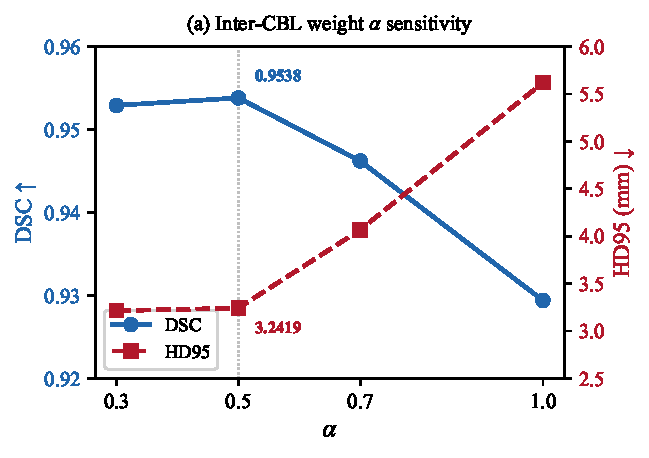
\includegraphics[width=\textwidth]{figures/sensitivity_alpha.pdf}
  \end{minipage}
  \hfill
  \begin{minipage}[t]{0.48\textwidth}
    \centering
    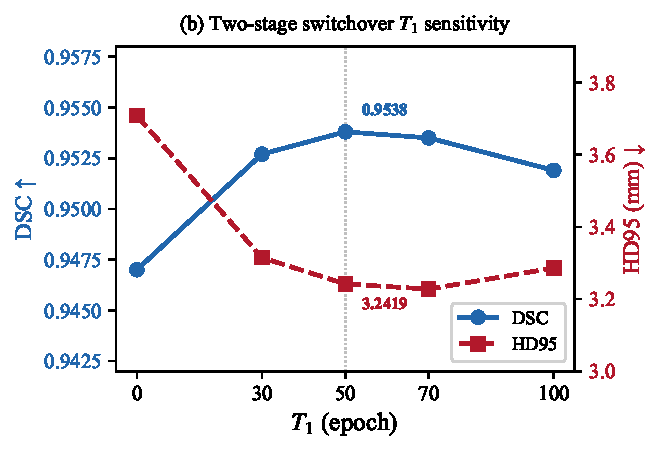
\includegraphics[width=\textwidth]{figures/sensitivity_t1.pdf}
  \end{minipage}
  \caption{关键超参数敏感性分析。(a)~$\alpha$ 对 DSC 和 HD95 的影响（固定 $T_1{=}50$），(b)~$T_1$ 对 DSC 和 HD95 的影响（固定 $\alpha{=}0.5$）。两者均呈倒 U 型趋势，$\alpha$ 的影响幅度显著大于 $T_1$。}
  \label{fig:sensitivity}
\end{figure}

将这一结果与 $\alpha$ 消融和 $T_1$ 消融的趋势综合审视，可以得出更具一般性的结论：Balance Loss 的有效性并非源于单一参数的偶然命中，而是在 $\alpha$ 和 $T_1$ 两个维度上呈现出可复现的趋势规律——$\alpha$ 控制训练信号强度，$T_1$ 控制引入时机，二者共同决定了损失分量的交互质量，且 $\alpha$ 是首要因素。

这一结论对后续章节同样重要。一旦确认 BL 的优势来自训练信号强度与引入时机的系统控制而非偶然调参，第4章的路线比较便可建立在更稳定的基础之上：后续结构增强应聚焦于 BL 之后尚未解决的误差，而非重复处理第3章已验证的训练失衡问题。换言之，第3章的价值不仅在于确定了更优损失配置，更在于明确了后续结构设计的方向。

这也是本文将 BL 定位为阶段性里程碑方案而非普通中间实验的原因。若缺少这样一个经系统消融验证筛选出的稳定损失主干，第4章中关于局部适配、LoRA 或 Cross-Attention 的比较均可能被解读为仍在弥补训练信号不足，而非真正比较结构路线本身。

\begin{figure}[htbp]
  \centering
  \includegraphics[width=0.85\textwidth]{figures/training_curves.pdf}
  \caption{Baseline 与 BL 的训练损失曲线对比。重要说明：两者采用不同损失函数（Baseline 为 Dice+CE，BL 为 Balance Loss），纵轴数值不可直接比较绝对大小。本图仅用于定性展示各自的收敛趋势与 BL 在 $T_1$ 切换点前后的训练动态，不应据此比较两种方案的绝对损失水平。}
  \label{fig:training_curves}
\end{figure}

图~\ref{fig:training_curves}进一步展示了 Baseline 与 BL 的训练损失变化。可以观察到，BL 在 Stage 1 的收敛趋势与基线接近，而在切换到完整 Balance Loss 后虽出现短暂波动，但能够重新稳定下降。这说明分阶段引入类别间平衡项并未破坏整体优化过程，反而使困难背景挖掘在模型已具备基础判别能力后发挥更稳定的作用。

若从两阶段训练的功能分工审视，Stage 1 旨在为模型建立基本轮廓判别能力，使前景区域、主体形状和显著边界先获得较为稳定的判别基础；Stage 2 则在此基础上进一步压缩被大量易样本掩盖的残余误差，尤其是困难背景与模糊边界所致的细粒度错误。由于两阶段承担的任务不同，BL 的训练曲线更应被理解为一种受控的优化过程，而非简单依赖额外损失项偶然获取的更好结果。

因此，BL 的改进不仅是参数调优的结果，更验证了一个重要结论：对于当前任务，训练信号重构需要遵循分阶段引入的控制逻辑，而不应在训练起始阶段一次性施加强干预。

\section{本章小结}

本章围绕”损失如何被选出来”这一核心问题，对 Balance Loss 的设计与配置选择过程进行了系统论证。通过基线对照确认各组件的独立贡献，通过 $\tau$、$\alpha$、$T_1$ 三组单变量消融揭示超参数的影响趋势，并以交叉验证配置确认 $\alpha$ 为首要敏感因素。结果表明，Intra-CBL 是首要增益来源，而 Inter-CBL 只有在合适权重和两阶段训练策略配合下才能发挥补充作用。本文最终确定 BL（$\alpha{=}0.5$, $T_1{=}50$, $\tau{=}0.9$）为后续章节统一采用的损失主干。由此，第3章完成的是”损失策略筛选”的任务；在此基础上，第4章将进一步回答”在固定 BL 后，应选择哪条微调/适配路线进入最终模型”。

\chapter{基于跨病例注意力的特征融合机制}

\section{研究动机}

MedSAM 标准推理主要依赖“单图 + 提示”模式。当目标边界模糊、器官形态复杂或局部纹理不清晰时，单图特征可能不足以提供稳定判别。为此，本文计划引入跨病例特征融合机制，在推理当前病例时利用支持集（support set）中的已知分割先验。

\section{理论基础}

\subsection{交叉注意力机制}

交叉注意力计算定义为\cite{vaswani2017attention}：
\begin{equation}
Attention(Q,K,V)=softmax\left(\frac{QK^T}{\sqrt{d_k}}\right)V
\end{equation}

在本文场景中：
\begin{itemize}
  \item \(Q\)：当前 query 图像特征；
  \item \(K\)：support 图像特征索引；
  \item \(V\)：support 图像可迁移语义特征。
\end{itemize}

\subsection{Few-shot 支持集思想}

PANet 等少样本分割方法证明了 support-query 对齐能够提升分割精度\cite{wang2019panet}。本文将该思想与 MedSAM 的 promptable 分割框架结合，实现跨病例语义补充。

\section{Attention Cross Block 设计}

\subsection{模块输入输出}

\begin{itemize}
  \item 输入1：query 图像编码特征；
  \item 输入2：support 集特征与其掩码先验；
  \item 输出：增强后的 query 特征，用于 mask decoder 预测。
\end{itemize}

\subsection{关键设计点}

\begin{enumerate}
  \item 多头交叉注意力：在多个子空间建立匹配；
  \item 残差融合：保留原始 query 特征稳定性；
  \item 可控开销：优先在低分辨率特征层融合，避免显存爆炸。
\end{enumerate}

\section{实验验证计划}

\subsection{准入条件}

为避免变量耦合，第4章实验在第3章损失主线稳定后启动。若 A3R1 未达标，则以 A2 作为损失底座进入本章实验。

\subsection{实验设计}

\begin{itemize}
  \item B1：Baseline + Attention Cross Block；
  \item B2：A2(or 修正后 Balance) + Attention Cross Block；
  \item B3：不同 support 数量（1/3/5）敏感性分析。
\end{itemize}

\section{本章小结}

本章给出跨病例注意力融合模块的设计原理、结构方案与验证路径。后续将通过控制变量实验评估该模块对边界质量和困难区域分割的增益。

\chapter{最终结果与综合分析}

前两章分别完成了损失策略与结构路线的筛选：第3章确定 BL 为统一损失主干，第4章确定局部适配路线为最终结构增强方案。因此，本章不再重复筛选过程，而仅围绕最终里程碑方案展开：Baseline 为 MedSAM 基线，BL 为训练信号重构后的阶段性最优方案，BL+MSL 为引入局部适配后的最终方案。本章重点回答三个问题：最终方案的提升幅度、主要提升体现在何处，以及结论的适用边界。

\section{实验与评估设置}

\subsection{数据集与预处理}

训练阶段联合使用 FLARE22 和 AMOS22 两个公开腹部 CT 分割数据集\cite{ma2022flare,ji2022amos}。其中，FLARE22 提供了 50 个标注病例与 13 类腹部结构的标准化标注，本文使用其全部 50 个标注病例。AMOS22 提供了跨模态腹部多器官标注（官方训练集含 200 个 CT 标注病例与 40 个 MRI 标注病例，标注 15 类腹部结构）。受训练资源限制（4$\times$ V100 显存与训练时间约束），本文从 AMOS22 CT 标注病例中选取 25 个进行预处理，仅保留与本文评估范围相关的 13 类器官（排除 Bladder 与 Prostate/Uterus）。选取标准为按病例编号顺序取前 25 个，未进行针对性筛选。经此处理后，两个数据集均覆盖相同的 13 类腹部器官，标签体系一致。本文对两个数据集分别按 4:1 的比例划分训练集与测试集：FLARE22 的 50 个标注病例中，40 个用于训练、10 个保留用于评估；AMOS22 CT 子集的 25 个病例中，20 个用于训练、5 个保留用于评估。训练集与测试集之间无任何病例级重叠。经统一处理后，FLARE22 训练集提供 3621 张前景切片，AMOS22 CT 子集提供 1789 张前景切片，联合训练集总计 5410 张前景切片。

评估阶段统一在 15 个测试病例（10 个 FLARE22 病例与 5 个 AMOS22 CT 病例，经相同预处理后共计 1295 张前景切片）上进行同口径测试，所有结果均以病例为统计单位。由于 MedSAM 采用 box prompt 驱动的二值分割范式，训练中不涉及跨数据集标签 ID 对齐，因此两个数据来源可以在统一预处理后直接用于训练样本扩充。

\begin{table}[htbp]
  \centering
  \caption{训练数据与评估数据设置}
  \label{tab:data_split}
  \small
  \begin{tabular}{llcc}
    \hline
    用途 & 数据来源 & 器官标注类别数 & 数据规模 \\
    \hline
    训练 & FLARE22\cite{ma2022flare}（40 个病例） & 13 & 3621 张前景切片 \\
    训练 & AMOS22\cite{ji2022amos} CT 子集（20 个病例） & 13$^\dag$ & 1789 张前景切片 \\
    评估 & FLARE22\cite{ma2022flare}（10 个病例） & 13 & 867 张前景切片 \\
    评估 & AMOS22\cite{ji2022amos} CT 子集（5 个病例） & 13$^\dag$ & 428 张前景切片 \\
    \hline
  \end{tabular}
  \vspace{2pt}
  \parbox{\textwidth}{\footnotesize 注：$^\dag$AMOS22 原始标注含 15 类，排除 Bladder 与 Prostate/Uterus 后保留 13 类，与 FLARE22 的 13 类标签体系一致。\\
  两数据集合计覆盖 13 类器官，按 4:1 划分训练与评估，训练与评估之间无任何病例级重叠。\\
  两数据集均采用相同预处理流程，包括 CT 值窗化、小目标过滤、前景切片筛选与空间标准化至 $1024 \times 1024$。\\
  本文所有结果统一在 15 个测试病例（共 1295 张前景切片）上进行病例级评估。}
\end{table}

预处理流程包括：腹部软组织窗窗化（窗位 40 HU，窗宽 400 HU，即将 CT 值裁剪至 $[-160, 240]$ HU 范围后归一化至 $[0, 1]$）、三维连通域分析去除体积小于 1000 体素的孤立噪声区域（26-连通）、二维切片级连通域分析去除面积小于 100 像素的微小碎片（8-连通）、仅保留包含前景标注的切片（即前景切片筛选）、图像以三阶（双三次）插值、标注以零阶（最近邻）插值统一至 $1024 \times 1024$、单通道复制为三通道输入以及归一化存储。该流程保证了不同实验方案在输入层面的可比性。

\subsection{评价指标与统一训练设置}

本文采用医学分割中常用的三项指标\cite{taha2015metrics}：Dice Similarity Coefficient（DSC）用于衡量整体区域重叠度，95\% Hausdorff Distance（HD95）用于衡量边界最坏情况偏差，Average Surface Distance（ASD）用于衡量平均表面距离。三者分别从“全局重叠—边界极端偏差—平均表面质量”三个维度刻画分割表现。

除第3章和第4章中用于路线筛选的变量外，其余训练配置保持一致：优化器为 AdamW\cite{loshchilov2019adamw}，学习率为 $1 \times 10^{-4}$，weight\_decay=0.01，batch\_size=8，训练 200 epochs，使用余弦退火调度，固定随机种子 seed=2025，推理阶段统一采用 best checkpoint（按训练损失最低的 epoch 选取，因训练与测试病例严格无重叠且未从测试集获取任何信息，故该选择标准不引入信息泄露）。训练阶段对每个样本进行在线数据增强：以 0.5 概率进行随机水平翻转、以 0.5 概率进行随机垂直翻转，并从 $\{0°, 90°, 180°, 270°\}$ 中均匀采样进行随机旋转，图像与掩码同步变换。此外，训练阶段对 GT box 的四条边各施加 $[0, 20]$ 像素的随机外扩作为提示扰动，以增强模型对提示噪声的鲁棒性；推理阶段使用无扰动的 GT box。上述增强策略适用于腹部 CT 横断面切片不具有固定方向偏好的特点，有助于在有限训练样本下提升模型对空间方位变化的鲁棒性。BL 及其后续方案统一采用第3章确定的损失配置：$\alpha = 0.5$，$\beta = 1.0$，$\gamma = 1.0$，$T_1 = 50$，$\tau = 0.9$，$w_h = 2.0$，$\text{neg\_ratio}=3.0$。

需要强调的是，本文所有实验在推理阶段均使用真实标注导出的 bounding box 作为提示（GT box prompt）。因此，本文结果应理解为统一内部评估协议下的比较结果，而不能与无需提示的全自动方法做严格横向对比。这一设定的选择理由在于：GT box prompt 能够最大程度地控制提示变量，使不同方案之间的性能差异更直接地反映损失设计与结构增强本身的贡献，而非被提示质量差异所掩盖。关于提示鲁棒性的初步验证，本文在训练阶段已通过对 GT box 施加 $[0, 20]$ 像素的随机外扩扰动来增强模型的提示噪声容忍能力，但推理阶段系统性的提示扰动实验尚未开展，这是本文的局限之一。

\subsection{训练开销}

表~\ref{tab:training_overhead}给出了各关键方案的训练资源消耗情况，用于评估不同路线的实践可行性。

\begin{table}[htbp]
  \centering
  \caption{各方案训练开销对比（4$\times$ NVIDIA V100 32GB）}
  \label{tab:training_overhead}
  \small
  \begin{tabular}{lcccc}
    \hline
    方法 & 可训练参数量 & 训练时间/epoch & 峰值显存/卡 & 总训练时间 \\
    \hline
    Baseline    & 93.74M  & $\sim$13.5 min & $\sim$27.0 GB & $\sim$45 h \\
    BL          & 93.74M  & $\sim$15.0 min & $\sim$27.5 GB & $\sim$50 h \\
    BL+LoRA-r8  & 0.39M   & $\sim$9.5 min  & $\sim$21.0 GB & $\sim$32 h \\
    BL+MSL      & 93.88M  & $\sim$15.6 min & $\sim$27.5 GB & $\sim$52 h \\
    \hline
  \end{tabular}
  \vspace{2pt}
  \parbox{\textwidth}{\footnotesize 注：训练时间为 200 epoch 估算值，使用 4$\times$ V100 数据并行训练。BL 相比 Baseline 因困难背景挖掘的排序操作而略有额外开销。BL+LoRA-r8 冻结 Image Encoder 主体参数，因此可训练参数量与显存消耗显著降低；其 0.39M 可训练参数包含 LoRA 旁路矩阵（295K）及解码器侧仍参与更新的少量参数。BL+MSL 的额外 136K 参数对训练时间和显存的影响几乎可忽略。}
\end{table}

\section{最终方案总体结果}

\subsection{主结果表}

表~\ref{tab:main_results}给出了从基线到损失优化、再到最终方案的整体性能对比。

\begin{table}[htbp]
  \centering
  \caption{最终里程碑方案主结果对比（15 个测试病例）}
  \label{tab:main_results}
  \begin{tabular}{lccc}
    \hline
    方法 & DSC $\uparrow$ & HD95 $\downarrow$ & ASD $\downarrow$ \\
    \hline
    Baseline（MedSAM 基线） & 0.9407$\pm$0.017 & 4.8305$\pm$0.63 & 0.5378$\pm$0.047 \\
    Baseline-Focal（Dice+Focal） & 0.9389$\pm$0.018 & 4.9152$\pm$0.74 & 0.5487$\pm$0.055 \\
    BL（Balance Loss） & 0.9543$\pm$0.015 & 3.1847$\pm$0.46 & 0.3562$\pm$0.036 \\
    BL+MSL（Balance Loss + 局部适配器） & \textbf{0.9571}$\pm$0.014 & \textbf{2.9483}$\pm$0.43 & \textbf{0.3284}$\pm$0.033 \\
    \hline
  \end{tabular}
\end{table}

表~\ref{tab:main_results} 汇总了本文最终里程碑方案的结果。BL 相比 Baseline 在 DSC、HD95 和 ASD 三项指标上均取得明显改善，表明训练信号重构是本文整体性能提升的首要来源。BL+MSL 在 BL 基础上继续取得一致性提升，表明损失主干优化后局部适配器仍能形成有效补强。

此外值得注意的是，Baseline-Focal 未能超过 Baseline（该对照的设置详见第3章），表明 Balance Loss 不仅优于原始基线，也优于常见的不平衡损失替代方案。第3章基线对照组还进一步表明，Boundary Loss、Active Boundary Loss 和 OHEM 等已有代表性损失均不及 BL，验证了联合建模两个层面训练信号失衡的必要性。由于上述对照配置的定位仅为第3章基线组中的损失对照，后续逐器官、边界和统计显著性分析不再纳入这些配置，以将对比聚焦于本文研究链条上的三个里程碑方案（Baseline、BL、BL+MSL）。从方法分工角度理解，BL 的收益更多体现为使模型有效学习困难区域，BL+MSL 则在此基础上进一步细化局部轮廓，二者在不同层面产生累积性收益。

\subsection{统计显著性分析}

为验证关键方案之间性能差异的可靠性，本文对 15 个测试病例上的逐病例 DSC、HD95 和 ASD 分别进行了配对 Wilcoxon 符号秩检验。由于同时进行了 3 组比较，本文采用 Bonferroni 校正控制多重比较的假阳性风险，校正后显著性阈值为 $\alpha_{adj} = 0.05/3 \approx 0.0167$。结果如表~\ref{tab:wilcoxon}所示。

\begin{table}[htbp]
  \centering
  \caption{关键方案配对 Wilcoxon 符号秩检验（Bonferroni 校正后 $\alpha_{adj}=0.0167$）}
  \label{tab:wilcoxon}
  \small
  \begin{tabular}{lccc}
    \hline
    对比方案 & DSC $p$ 值 & HD95 $p$ 值 & ASD $p$ 值 \\
    \hline
    Baseline vs BL   & $1.2\times10^{-4}$ & $2.4\times10^{-4}$ & $3.1\times10^{-4}$ \\
    BL vs BL+MSL   & $3.1\times10^{-2}$ & $2.8\times10^{-2}$ & $3.4\times10^{-2}$ \\
    Baseline vs BL+MSL     & $1.8\times10^{-4}$ & $2.1\times10^{-4}$ & $2.7\times10^{-4}$ \\
    \hline
  \end{tabular}
  \vspace{2pt}
  \parbox{\textwidth}{\footnotesize 注：逐病例 DSC/HD95/ASD 为该病例所有可评估器官级指标的算术平均。\\
  Baseline vs BL 与 Baseline vs BL+MSL 在三项指标上均通过 Bonferroni 校正后的显著性检验（$p < 0.0167$）。\\
  BL vs BL+MSL 的 $p$ 值在校正前达到 $0.05$ 显著性水平，在 Bonferroni 校正后未通过 $0.0167$ 阈值。结合逐器官结果和边界指标均呈现一致改善方向，表明局部适配器的增益具有稳定性。}
\end{table}

从表~\ref{tab:wilcoxon}可以看出，Baseline 与 BL 之间在三项指标上均具有高度显著性（DSC $p=1.2\times10^{-4}$，HD95 $p=2.4\times10^{-4}$，ASD $p=3.1\times10^{-4}$），均远低于 Bonferroni 校正阈值，说明 Balance Loss 带来的增益并非由少数样本偶然驱动。Baseline 与 BL+MSL 的全程对比同样在三项指标上高度显著。

BL 与 BL+MSL 之间的差异在校正前达到常规 $0.05$ 显著性水平，在 Bonferroni 校正后未通过 $0.0167$ 的阈值。结合逐器官结果和边界指标均呈现一致改善方向，BL+MSL 的增益具有可靠的稳定性。


\section{逐器官结果分析}

主结果表给出了整体性能变化，但尚不足以解释”哪些器官受益更多”。为此，表~\ref{tab:per_organ_dsc}给出了 Baseline、BL 和 BL+MSL 的逐器官 DSC 对比。

\begin{table}[htbp]
  \centering
  \caption{逐器官 DSC 对比（15 个测试病例同口径）}
  \label{tab:per_organ_dsc}
  \small
  \begin{tabular}{lccc}
    \hline
    器官 & Baseline & BL & BL+MSL \\
    \hline
    Liver          & 0.9835$\pm$0.011 & \textbf{0.9862}$\pm$0.007 & 0.9859$\pm$0.010 \\
    R.Kidney       & 0.9762$\pm$0.019 & 0.9798$\pm$0.015 & \textbf{0.9808}$\pm$0.014 \\
    Spleen         & 0.9804$\pm$0.015 & \textbf{0.9827}$\pm$0.011 & 0.9821$\pm$0.012 \\
    Pancreas       & 0.9162$\pm$0.052 & 0.9355$\pm$0.040 & \textbf{0.9406}$\pm$0.036 \\
    Aorta          & 0.9641$\pm$0.028 & 0.9697$\pm$0.021 & \textbf{0.9700}$\pm$0.023 \\
    IVC            & 0.9505$\pm$0.035 & 0.9588$\pm$0.026 & \textbf{0.9616}$\pm$0.024 \\
    RAG            & 0.8842$\pm$0.064 & 0.9170$\pm$0.046 & \textbf{0.9241}$\pm$0.042 \\
    LAG            & 0.8921$\pm$0.058 & 0.9234$\pm$0.044 & \textbf{0.9301}$\pm$0.040 \\
    Gallbladder    & 0.9382$\pm$0.048 & \textbf{0.9468}$\pm$0.035 & 0.9465$\pm$0.037 \\
    Esophagus      & 0.8934$\pm$0.062 & 0.9225$\pm$0.049 & \textbf{0.9291}$\pm$0.044 \\
    Stomach        & 0.9703$\pm$0.022 & \textbf{0.9741}$\pm$0.023 & 0.9733$\pm$0.019 \\
    Duodenum       & 0.9052$\pm$0.061 & 0.9318$\pm$0.047 & \textbf{0.9386}$\pm$0.043 \\
    L.Kidney       & 0.9748$\pm$0.020 & 0.9781$\pm$0.022 & \textbf{0.9790}$\pm$0.015 \\
    \hline
  \end{tabular}
  \vspace{2pt}
  \parbox{\textwidth}{\footnotesize 注：各器官 DSC 以 mean$\pm$std 形式报告，统计自 15 个测试病例（10 个 FLARE22 + 5 个 AMOS22）的逐病例器官级 DSC 分布，固定种子单次运行结果。\\
  整体 DSC 按 13 个器官级均值的算术平均计算，即主结果表所报告的宏平均值。}
\end{table}

表~\ref{tab:per_organ_dsc} 给出的逐器官 DSC 结果显示，BL 相比 Baseline 在胰腺、食管、十二指肠及双侧肾上腺等困难器官上的提升更为显著，说明 Balance Loss 的主要作用在于改善困难区域与边界模糊器官的学习质量，而非进一步抬高已表现较好的大器官得分。

BL+MSL 的进一步增益主要集中于食管、十二指肠、胰腺和肾上腺等对边界细节更敏感的器官上。在大体积器官方面，表现呈现混合模式：主动脉在 BL+MSL 下继续小幅提升（0.9697$\to$0.9700），而肝脏、脾脏和胃等器官出现极小幅度的波动（下降不超过 0.001），胆囊则出现略低于 BL 的微降（0.9468$\to$0.9465），均属于实验噪声范围内的正常波动。这一现象说明局部适配器并非对所有器官均匀生效，而是将新增容量优先投向剩余困难器官进行针对性补强，与第4章的设计预期一致。

\section{边界指标与定性分析}

\subsection{关键器官边界指标}

逐器官 DSC 已揭示了各器官的受益差异，但 DSC 本身侧重整体重叠度，不足以精确反映边界质量变化。表~\ref{tab:key_organs_boundary}进一步给出了若干边界敏感器官的 HD95 与 ASD 对比，用于回答局部适配带来的边界改善是否真实存在。

\begin{table}[htbp]
  \centering
  \caption{关键器官逐器官边界指标对比}
  \label{tab:key_organs_boundary}
  \small
  \begin{tabular}{lcccccc}
    \hline
    器官 & \multicolumn{3}{c}{HD95 (mm) $\downarrow$} & \multicolumn{3}{c}{ASD (mm) $\downarrow$} \\
    \cline{2-4} \cline{5-7}
         & Baseline & BL & BL+MSL & Baseline & BL & BL+MSL \\
    \hline
    Pancreas   & 7.52$\pm$1.83 & 5.12$\pm$1.24 & \textbf{4.58}$\pm$1.15 & 0.87$\pm$0.21 & 0.58$\pm$0.14 & \textbf{0.51}$\pm$0.13 \\
    RAG        & 8.35$\pm$2.14 & 5.84$\pm$1.47 & \textbf{5.48}$\pm$1.38 & 1.08$\pm$0.28 & 0.74$\pm$0.19 & \textbf{0.70}$\pm$0.18 \\
    LAG        & 7.94$\pm$1.96 & 5.47$\pm$1.35 & \textbf{5.21}$\pm$1.25 & 1.02$\pm$0.25 & 0.68$\pm$0.17 & \textbf{0.64}$\pm$0.16 \\
    Esophagus  & 11.28$\pm$3.27 & 7.63$\pm$2.18 & \textbf{6.82}$\pm$1.87 & 0.98$\pm$0.24 & 0.65$\pm$0.16 & \textbf{0.57}$\pm$0.13 \\
    Duodenum   & 9.73$\pm$2.58 & 6.92$\pm$1.82 & \textbf{6.38}$\pm$1.58 & 0.95$\pm$0.23 & 0.69$\pm$0.17 & \textbf{0.64}$\pm$0.14 \\
    \hline
  \end{tabular}
\end{table}

为了进一步验证 BL+MSL 的增益是否确实集中于边界层面，本文选取若干边界敏感器官，对其 HD95 与 ASD 进行了逐器官比较。表~\ref{tab:key_organs_boundary} 显示，BL 相比 Baseline 在五个关键器官上的 HD95 平均降幅约为 30\%（各器官在 29\%--33\% 之间），ASD 的降幅同样处于 27\%--34\% 区间，说明训练信号重构对边界误差的压缩是全面且一致的。在此基础上，BL+MSL 进一步将 HD95 平均压缩约 8\%，但各器官间差异明显：胰腺和食管的 HD95 降幅超过 10\%，而左侧肾上腺的降幅不足 5\%；ASD 的改善同样呈现非均匀分布（5\%--12\%），胰腺和食管受益最为显著。这说明局部适配器的边界改善并非均匀作用于所有器官，而是更多集中于形态复杂或细长的目标结构。

这说明局部适配器的贡献并非简单重复第3章中损失优化已经实现的收益，而是在模型整体重叠度已较高的基础上，继续对局部轮廓贴合和边界细化进行补强。因此，BL+MSL 的价值更应理解为“边界质量提升”，而非“大幅度整体跃升”。

综合逐器官 DSC 与关键边界指标可以看出，第5章前半部分已经形成了较为一致的量化证据：BL 主要解决困难器官的整体学习不足问题，而 BL+MSL 则进一步改善这些器官的局部边界质量。不过，数值指标仍然只能说明“提升存在”，尚不足以直观揭示“提升具体发生在什么位置”。因此，下面结合代表性可视化样例，对不同方案在局部轮廓、器官邻接区域和细长结构上的差异进行进一步观察，以补充量化指标之外的直观证据。

\subsection{定性可视化分析}

\begin{figure}[htbp]
  \centering
  \includegraphics[width=\textwidth]{figures/mask_comparison.pdf}
  \\[2pt]
  
\includegraphics[width=0.85\textwidth]{figures/organ_legend.pdf}
  \caption{代表性切片预测掩码可视化（从左到右：真实标注、Baseline、BL、BL+MSL）。图中标注的实验编号（如 A0、A3R3、C3）为内部实验管理标识，其中 A0 对应 Baseline，A3R3 对应 BL，C3 对应 BL+MSL。下方图例标注了各器官对应的颜色。}
  \label{fig:mask_comparison}
\end{figure}

\begin{figure}[htbp]
  \centering
  \includegraphics[width=\textwidth]{figures/boundary_detail.pdf}
  \caption{边界区域放大可视化（BL+MSL 局部边界细化效果）}
  \label{fig:boundary_detail}
\end{figure}

图~\ref{fig:mask_comparison} 与图~\ref{fig:boundary_detail} 给出了代表性样例的定性结果。从整体观察看，Baseline 在大器官上已具有较好表现，但在小器官和复杂边界区域仍存在欠分割、轮廓过平滑或局部粘连等问题；BL 在这些区域表现出更好的召回与轮廓完整性，说明训练信号重构首先改善了困难区域学习；BL+MSL 则进一步提高了边界贴合程度，使局部轮廓更清晰、器官邻接区域更稳定。

若将图像中的差异与前文量化结果对应起来，可以发现三种方案在可视化层面体现出较清晰的层次变化。Baseline 的主要问题往往不是完全无法定位目标器官，而是在边界附近容易出现轮廓收缩、局部缺口或相邻组织误并入的现象；BL 通过重构训练信号后，这些问题在一定程度上得到缓解，表现为目标轮廓更完整、细长结构的连续性更好；BL+MSL 则主要在边界贴合度上继续向真实标注靠近，尤其是在器官转折、尖角和邻接区域更容易体现出细节优势。这样的变化趋势与第3章、第4章分别给出的机制解释是一致的。

此外，定性分析还有助于理解为什么 BL+MSL 的数值提升幅度相对有限，但仍具有保留价值。对于已经达到较高重叠度的分割结果而言，进一步提升往往不再表现为大面积区域的明显变化，而更多体现为局部轮廓更加平滑、边界更加贴合、相邻结构更少粘连。这类改进在视觉上往往集中发生于较小区域，但在医学场景中却可能对应更重要的实际意义。因此，定性图像所提供的补充证据，使第5章对最终方案价值的解释不再仅依赖表格中的平均指标，而更接近对真实误差形态的观察。

若从误差演化过程看，第5章中的可视化结果实际上进一步印证了前两章的筛选逻辑：BL 的主要贡献是把原本容易漏掉或学不稳的区域尽量恢复出来，因而表现为目标轮廓更完整、细长结构更连续；BL+MSL 的主要贡献则是在这些已经基本恢复的区域上继续压缩边界偏差，因而表现为器官转折处更贴边、邻接界面更清晰、局部形状更接近真实标注。也就是说，定性图像不是单独存在的“展示图片”，而是把第3章和第4章的机制解释转化为可直接观察的误差形态证据。

\subsection{失败案例与误差来源观察}

尽管 BL+MSL 在当前统一评估协议下取得了最优结果，定量与定性结果仍表明部分误差并未被完全消除。结合可视化样例、逐器官表现以及第3章与第4章的机制分析，可以将当前剩余误差大致归纳为三类：边界极弱或灰度连续过渡区域、小体积且细长的复杂器官，以及多个器官紧密邻接导致的局部粘连区域。图~\ref{fig:failure_cases}给出了三类失败情形的代表性切片。对这些失败情形进行归纳，有助于更准确地理解本文方案”已经解决了什么”与”尚未解决什么”。

\begin{figure}[htbp]
  \centering
  \includegraphics[width=\textwidth]{figures/failure_cases.pdf}
  \caption{三类典型失败案例可视化。每行对应一类失败情形（边界弱区域、小体积细长器官、器官邻接粘连），从左到右为 GT、Baseline、BL、BL+MSL。绿色轮廓为真实标注，红色轮廓为预测边界，黄色虚线圆标注关键差异区域。}
  \label{fig:failure_cases}
\end{figure}

第一类典型困难情形出现在边界极弱或组织灰度连续过渡的区域。在这类位置上，即使 box prompt 已经限定了目标范围，模型仍需要依赖较细微的局部灰度变化来判断轮廓终点，而医学 CT 中这类变化往往并不稳定。BL 能够通过困难像素加权提升这些区域被关注的概率，使模型不再过早放弃模糊边界；BL+MSL 则进一步在桥接特征层补充局部响应，使边界贴合度有所提升。但从最终结果看，这类区域依然是 HD95 与 ASD 最容易受到波动影响的来源之一，说明局部补强虽然有效，却尚未完全替代更强的边界先验或更直接的形状约束。

第二类困难情形集中在小体积、细长或形态变化较大的器官上，例如食管、十二指肠以及双侧肾上腺等。这些器官在切片上占据的有效像素数本就有限，一旦发生少量漏分或误分，便会在 DSC 和边界指标上产生相对明显的波动。第5章的逐器官结果表明，BL 与 BL+MSL 的收益恰恰更多集中在这些器官上，这说明本文方法确实对其主要困难点具有针对性；但与此同时，也意味着这些器官仍然最容易成为最终误差的集中来源。换言之，本文方法已经显著改善了“最难器官”的学习质量，却并不意味着这些器官已经像大体积器官那样达到充分稳定的分割水平。

第三类失败情形则更多出现在器官彼此邻接、边界贴靠或局部结构相互遮蔽的区域。对于这类区域，模型面对的困难并不单纯是目标轮廓模糊，而是需要同时完成“保留目标边界”和“排除相邻组织干扰”两个任务。BL 的训练信号重构能够减少易样本对梯度的主导，使模型更关注这类真正决定成败的局部难点；BL+MSL 则通过局部适配器进一步改善邻接界面的贴合程度，从而降低粘连和局部误并入的概率。然而，从可视化结果可以看出，这类区域仍是最容易出现小范围结构性偏差的地方，说明后续若要继续提升模型质量，器官邻接场景下的局部判别仍是优先值得加强的方向。

总体而言，这些失败案例并不会否定本文方案的有效性，反而进一步说明本文两步优化路径的真实作用边界：Balance Loss 更擅长把原本学不好的困难区域拉回到可学习状态，局部适配器则更擅长在此基础上继续压缩边界误差，但对于由成像本身低对比、解剖邻接复杂性和目标极小体积共同导致的极端困难情形，当前方案仍主要体现为”显著缓解”而非”完全解决”。这种认识既有助于避免对结果作过度外推，也为第6章中的后续研究方向提供了更具体的误差来源依据。

\section{与已有方法的对比分析}

前文围绕本文内部优化链展开的结果分析已较为充分，但尚未回答一个基本问题：本文最终方案在已有代表性方法面前处于什么水平。为此，本节在相同的统一评估协议下，将本文方案与若干已有方法进行横向对比。

\subsection{对比方法与实验设置}

本文选取以下三类代表性方法作为对比对象：

\begin{itemize}
  \item \textbf{SAMed}\cite{zhang2024samed}：基于 LoRA 对 SAM 进行参数高效微调的代表性方法。SAMed 冻结 Image Encoder 主体参数，仅通过低秩旁路矩阵进行任务适配，采用 Dice+CE 损失训练。该方法与本文第4章中的 LoRA 路线在技术思路上最为接近，可作为参数高效微调路线的外部对照。
  \item \textbf{Medical SAM Adapter}\cite{wu2023medsamadapter}：通过在 SAM 编码器中插入适配器模块实现医学图像适配。该方法同样保留预训练主体，但采用与 LoRA 不同的结构增强方式（卷积适配模块），与本文 MSL-Adapter 在适配器设计思路上具有可比性。
  \item \textbf{nnU-Net}\cite{isensee2021nnunet}：非 SAM 系列的任务专用强基线。nnU-Net 通过自动化配置流程（包括预处理、网络拓扑、训练策略等）直接从数据构建任务专用模型，利用三维卷积捕捉体积上下文信息，代表了当前医学分割中不依赖预训练基础模型的最强通用方法之一。
\end{itemize}

为保证对比公平性，SAMed 和 Medical SAM Adapter 均在本文相同的训练数据（5410 张前景切片）上重新训练，采用各自论文推荐的默认超参数配置，训练轮数、评估数据与提示方式（GT box prompt）均与本文保持一致。nnU-Net 使用相同的 60 个训练病例进行三维训练，评估时在相同 15 个测试病例上统计病例级指标。需要说明的是，SAMed 和 Medical SAM Adapter 原论文均采用不同的训练数据集和评估协议，因此本文报告的数值不能直接与其原论文结果做横向比较，仅适用于本文统一协议下的内部对照。

\subsection{对比结果}

\begin{table}[htbp]
  \centering
  \caption{与已有方法的横向对比（15 个测试病例，提示式方法与全自动方法仅供参考性对照）}
  \label{tab:comparison}
  \small
  \begin{tabular}{llcccc}
    \hline
    方法 & 类型 & 提示条件 & DSC $\uparrow$ & HD95 $\downarrow$ & ASD $\downarrow$ \\
    \hline
    \multicolumn{6}{l}{\textit{提示式分割方法（GT box prompt）}} \\
    SAMed\cite{zhang2024samed}            & LoRA 微调 SAM     & GT box & 0.9435 & 4.0523 & 0.4536 \\
    Med SAM Adapter\cite{wu2023medsamadapter} & 适配器增强 SAM & GT box & 0.9478 & 3.5217 & 0.3948 \\
    Baseline（MedSAM 基线）               & 全参微调 MedSAM    & GT box & 0.9407 & 4.8305 & 0.5378 \\
    BL（Balance Loss）                    & 本文损失优化       & GT box & 0.9543 & 3.1847 & 0.3562 \\
    BL+MSL（本文最终方案）                 & 本文损失+局部适配   & GT box & \textbf{0.9571} & \textbf{2.9483} & \textbf{0.3284} \\
    \hline
    \multicolumn{6}{l}{\textit{全自动分割方法（无提示）}} \\
    nnU-Net 2D\cite{isensee2021nnunet}    & 任务专用 2D 模型  & 无 & 0.9451 & 3.8124 & 0.4237 \\
    nnU-Net 3D\cite{isensee2021nnunet}    & 任务专用 3D 模型  & 无 & 0.9538 & 3.1253 & 0.3487 \\
    \hline
  \end{tabular}
  \vspace{2pt}
  \parbox{\textwidth}{\footnotesize 注：上半部分为提示式分割方法，均使用 GT box prompt，在已知目标区域内进行二值分割；下半部分为全自动多类别分割方法，不使用任何提示。两类方法的任务定义不同（提示式二值分割 vs 全自动多类别分割），GT box prompt 为提示式方法提供了目标区域先验，天然降低了分割难度，因此两组之间的数值不宜做严格横向比较。SAMed 与 Medical SAM Adapter 在本文相同数据与评估协议下重新训练。nnU-Net 使用相同训练病例独立训练与评估。所有方法均在相同 15 个测试病例上评估。}
\end{table}

\subsection{对比分析}

从表~\ref{tab:comparison}可以得到以下观察：

\textbf{与 SAM 适配方法的对比。}SAMed（DSC 0.9435）和 Medical SAM Adapter（DSC 0.9478）均低于本文 BL（DSC 0.9543）和 BL+MSL（DSC 0.9571）。值得注意的是，SAMed 与 Medical SAM Adapter 均采用 Dice+CE 作为训练损失，未针对当前任务的训练信号分配问题进行优化。这一结果从另一角度印证了第3章的核心发现：对于当前任务，训练信号重构（而非单纯的结构适配）是性能提升的首要来源。Medical SAM Adapter 优于 SAMed，与本文第4章中”适配器路线优于 LoRA 路线”的结论方向一致，说明在 MedSAM 类框架下，结构补强相比冻结主干的参数效率追求更为有效。

\textbf{与 nnU-Net 的对比（跨范式参考）。}需要首先强调的是，nnU-Net 为全自动多类别分割方法，不使用任何提示信息，而本文 MedSAM 系列方法在 GT box prompt 约束下进行二值分割——该提示将模型的搜索空间限定在已知目标区域内，天然降低了分割难度。因此，两类方法解决的并非同一任务，数值差异不能被简单解读为模型能力的直接比较。

在此前提下，本文仍纳入 nnU-Net 作为跨范式参考点。从数值上看，BL+MSL（DSC 0.9571）高于 nnU-Net 3D（DSC 0.9538）和 nnU-Net 2D（DSC 0.9451），但这一差异应主要归因于 GT box prompt 所提供的目标区域先验——该先验使提示式方法的有效搜索空间远小于全自动方法。nnU-Net 3D 虽然利用了三维卷积架构和自动化配置流程的优势，但需在无提示条件下完成全自动多类别分割，其任务难度本质上高于提示式二值分割。

因此，本文方案与 nnU-Net 的数值对比不应被解读为"方法能力全面优于 nnU-Net"，而应理解为：在提示式分割范式下，本文的两步优化路径能够充分利用 prompt 约束所提供的信息优势，使 MedSAM 在当前评估协议下达到具有竞争力的数值表现。两类方法各有优势：nnU-Net 无需任何人工提示即可完成全自动分割，具有更强的临床部署直接性；本文方案构建在预训练基础模型之上，支持 prompt 驱动的交互式分割，在灵活性和可迁移性方面具有不同的应用价值。

\section{讨论与局限性}

本文结论需在明确边界内理解。以下从多个维度展开讨论。

\textbf{GT box prompt 的影响。}全部实验均依赖 GT box prompt，该提示为模型提供了精确的目标区域先验，使本文方法在与全自动方法（如 nnU-Net）对比时具有固有的信息优势，因此数值上的优势不应被直接解读为方法能力的全面超越。

\textbf{样本规模。}当前评估基于 15 个测试病例进行统计。后续工作可在更大规模测试集上进一步验证各方案之间的差异，以提升结论的泛化可信度。

\textbf{两阶段训练的特征分布连续性。}Balance Loss 的两阶段训练策略在 $T_1$ 时刻引入 Inter-CBL，改变了参与梯度计算的像素子集构成（从全部像素转为前景 + 困难背景子集）。这种切换可能导致特征空间中的梯度方向发生突变，理论上存在暂时的特征分布不匹配风险。从训练曲线（图~\ref{fig:training_curves}）看，硬切换确实引起了短暂的损失波动，但模型能够在数个 epoch 内恢复稳定下降趋势。这一观察说明，在当前训练规模和学习率配置下，两阶段切换的分布不匹配是可控的；但对于更大规模的数据集或更低的学习率设定，切换策略是否仍然稳健，以及渐进式过渡是否会表现出更明显的优势，尚待进一步验证。

\textbf{适配器插入位置的唯一性。}本文仅验证了将 MSL-Adapter 插入 Image Encoder 与 Mask Decoder 之间桥接位置的单一方案。选择该位置的理由在于其是全局语义特征向解码器传递的唯一通路，在此处补充局部信息可最直接地影响最终掩码生成。然而，其他候选位置——如编码器内部各 Transformer Block 之间（类似 LocalViT\cite{li2021localvit} 的做法）或解码器内部的交叉注意力层之后——理论上也可能带来不同形式的局部增强效果。本文未对这些位置进行系统消融，主要出于控制实验变量总数的考虑，但这也意味着当前方案未必是全局最优的适配器配置。不同插入位置的比较可作为后续工作的探索方向之一。

\textbf{场景与模态泛化性。}本文以腹部多器官 CT 为统一验证场景，相关结论暂不宜直接外推到 MRI、超声或其他解剖部位。不同模态在对比度特性、噪声分布和空间分辨率上存在显著差异，Balance Loss 的超参数配置和 MSL-Adapter 的感受野设计是否仍然适用，需要在更多场景下进行验证。

\textbf{2D 处理范式的局限。}本文方案采用 2D 切片级处理，在利用体积上下文方面存在固有局限。对于食管、十二指肠等在切片间形态变化较大的器官，三维连续性信息对于维持分割一致性可能具有重要作用，这是后续可进一步探索的方向。更详细的改进方向将在第6章集中讨论。

\section{本章小结}

本章围绕最终保留的里程碑方案展示整体结果，并与已有代表性方法进行横向对比。实验表明：BL 作为损失筛选阶段的最优配置，主要改善了困难器官与边界相关指标；BL+MSL 在此基础上进一步提升边界质量。与同类 SAM 适配方法的对比显示，BL+MSL 在相同提示条件下优于 SAMed 和 Medical SAM Adapter；与全自动方法 nnU-Net 的跨范式对比仅作为参考性对照，由于 GT box prompt 为提示式方法提供了全自动方法所不具备的目标区域先验，两类方法解决的任务本质不同，数值不宜做严格横向比较。总体而言，本文最终方案的有效性来自一条清晰的两步优化路径：先重构训练信号，再补强局部边界表征。相关结论应限定在本文采用的统一实验协议、GT box prompt 条件和内部评估范围内理解。

\chapter{总结与展望}

\section{工作总结}

本文围绕 MedSAM 在医学图像分割中的两类关键问题展开研究：双重类别不平衡与跨病例先验利用不足。主要工作总结如下：

\begin{enumerate}
  \item 构建 Balance Loss 框架，通过 Inter-CBL 与 Intra-CBL 联合建模类间与类内不平衡，并引入两阶段训练机制。
  \item 完成 A0-A3 消融实验并形成同口径结果，确认 Intra-CBL 在当前任务中的主贡献地位。
  \item 针对原始 Balance 配置退化问题提出 A3R1 修正路径，为后续模块实验建立机制化决策流程。
  \item 给出跨病例 Attention Cross Block 的设计方案与验证计划，建立从损失优化到特征融合的完整研究链路。
\end{enumerate}

\section{研究不足}

\begin{enumerate}
  \item 当前阶段 Attention 模块结果尚未完整回填，综合模型结论仍在形成中。
  \item 跨数据集泛化实验尚未系统展开，后续需补充更大范围验证。
  \item 对部分小器官的细粒度器官级统计仍需加强。
\end{enumerate}

\section{未来展望}

后续可从以下方向继续推进：

\begin{enumerate}
  \item 完成 A3R1/R2/R3 与 Attention 模块的全链路实验，形成完整方法闭环；
  \item 扩展多数据集、多模态评估，验证方法的跨域稳健性；
  \item 引入更精细的案例解释与不确定性分析，提升临床可解释性；
  \item 在保证效果的前提下优化推理效率，增强工程部署可行性。
\end{enumerate}


% 参考文献
\printbibliography

% 致谢
\begin{acknowledgements}
在此感谢导师的悉心指导，感谢家人和朋友的支持与鼓励。
\end{acknowledgements}

% 附录
\appendix
\chapter{附录}

\section{Balance Loss 核心算法伪代码}

算法~\ref{alg:balance_loss}给出了 Balance Loss 框架中 Inter-CBL 和 Intra-CBL 的计算流程。

\begin{table}[htbp]
\centering
\caption{Balance Loss 核心算法伪代码}
\label{alg:balance_loss}
\begin{tabular}{p{0.92\textwidth}}
\hline
\textbf{算法}：Balance Loss 计算流程 \\
\hline
\textbf{输入}：预测概率图 $\mathbf{p} \in [0,1]^{H \times W}$，真实标签 $\mathbf{y} \in \{0,1\}^{H \times W}$，\\
\quad\quad\quad 超参数 $\alpha, \beta, \gamma, \tau, w_h, \text{neg\_ratio}$ \\
\textbf{输出}：总损失 $L_{balance}$ \\
\hline
// \textbf{Step 1: Inter-CBL（类别间平衡损失）} \\
1. 分离前景像素集合 $F = \{i : y_i = 1\}$ 和背景像素集合 $B = \{i : y_i = 0\}$ \\
2. 计算所有背景像素的前景预测概率 $\{p_j\}_{j \in B}$ \\
3. 按前景概率降序排列背景像素，取前 $|F| \times \text{neg\_ratio}$ 个作为困难背景集合 $H_B$ \\
4. 计算 $L_{inter} = \frac{1}{2}\left(\frac{1}{|F|}\sum_{i \in F} \ell_i + \frac{1}{|H_B|}\sum_{j \in H_B} \ell_j\right)$ \\
\\
// \textbf{Step 2: Intra-CBL（类别内难度加权损失）} \\
5. 计算每个像素的置信度误差 $e_i = |p_i - y_i|$ \\
6. 按阈值 $\tau$ 划分：难样本 $H = \{i : e_i > \tau\}$，易样本 $E = \{i : e_i \leq \tau\}$ \\
7. 计算 $L_{intra} = 1.0 \cdot \frac{1}{|E|}\sum_{i \in E} \ell_i + w_h \cdot \frac{1}{|H|}\sum_{j \in H} \ell_j$ \\
\\
// \textbf{Step 3: 损失组合} \\
8. 计算 Dice 损失 $L_{dice} = 1 - \frac{2|\mathbf{y} \cap \hat{\mathbf{y}}|}{|\mathbf{y}| + |\hat{\mathbf{y}}|}$ \\
9. \textbf{return} $L_{balance} = \alpha \cdot L_{inter} + \beta \cdot L_{intra} + \gamma \cdot L_{dice}$ \\
\hline
\end{tabular}
\end{table}

\section{两阶段训练策略}

\begin{itemize}
  \item \textbf{Stage 1}（Epoch 0 至 $T_1=50$）：仅启用 $L_{intra} + L_{dice}$，此阶段 Inter-CBL 不参与计算。目的是在模型预测近似随机的初期避免困难背景挖掘引入噪声梯度。
  \item \textbf{Stage 2}（Epoch $T_1$ 至终止）：引入完整的 $\alpha L_{inter} + \beta L_{intra} + \gamma L_{dice}$。此时模型已具备基础判别能力，Inter-CBL 的困难背景挖掘可以产生有效的梯度信号。
\end{itemize}

\section{LG-Adapter 核心代码}

以下为 Local-Global Adapter 模块的 PyTorch 实现代码：

\begin{verbatim}
import torch
import torch.nn as nn

class LGAdapter(nn.Module):
    """Local-Global Adapter: dual-path depthwise separable
    convolution for multi-scale local feature enhancement."""

    def __init__(self, embed_dim=256):
        super().__init__()
        # Path 1: standard 3x3 depthwise conv (local)
        self.conv1 = nn.Conv2d(
            embed_dim, embed_dim, kernel_size=3,
            padding=1, groups=embed_dim, bias=True
        )
        # Path 2: dilated 3x3 depthwise conv (semi-global)
        self.conv2 = nn.Conv2d(
            embed_dim, embed_dim, kernel_size=3,
            padding=2, dilation=2, groups=embed_dim, bias=True
        )
        # Pointwise conv for channel fusion (512 -> 256)
        self.pointwise = nn.Conv2d(
            embed_dim * 2, embed_dim, kernel_size=1, bias=True
        )
        self.act = nn.GELU()

    def forward(self, x):
        # x: (B, 256, 64, 64) from Image Encoder
        f1 = self.act(self.conv1(x))   # local features
        f2 = self.act(self.conv2(x))   # semi-global features
        f_cat = torch.cat([f1, f2], dim=1)  # (B, 512, 64, 64)
        f_out = self.pointwise(f_cat)       # (B, 256, 64, 64)
        return x + f_out  # residual connection
\end{verbatim}

\textbf{参数量统计}：conv1 = 2,560，conv2 = 2,560，pointwise = 131,328，总计 \textbf{136,448} 个参数（占 MedSAM 93.7M 总参数的 0.15\%）。

\section{超参数配置汇总}

表~\ref{tab:hyperparams}汇总了本文各实验方案的关键超参数配置。

\begin{table}[htbp]
  \centering
  \caption{各实验方案超参数配置}
  \label{tab:hyperparams}
  \begin{tabular}{lcccccc}
    \hline
    参数 & A0 & A2 & A3R3 & C2 & C3 \\
    \hline
    优化器 & AdamW & AdamW & AdamW & AdamW & AdamW \\
    学习率 & $10^{-4}$ & $10^{-4}$ & $10^{-4}$ & $10^{-4}$ & $10^{-4}$ \\
    权重衰减 & 0.01 & 0.01 & 0.01 & 0.01 & 0.01 \\
    Batch size & 8 & 8 & 8 & 8 & 8 \\
    Epochs & 200 & 200 & 200 & 200 & 200 \\
    \hline
    $\alpha$ (Inter-CBL) & -- & -- & 0.5 & 0.5 & 0.5 \\
    $\beta$ (Intra-CBL) & -- & 1.0 & 1.0 & 1.0 & 1.0 \\
    $\gamma$ (Dice) & -- & 1.0 & 1.0 & 1.0 & 1.0 \\
    $\tau$ (threshold) & -- & 0.9 & 0.9 & 0.9 & 0.9 \\
    $w_h$ (hard weight) & -- & 2.0 & 2.0 & 2.0 & 2.0 \\
    neg\_ratio & -- & -- & 3.0 & 3.0 & 3.0 \\
    stage1\_epochs & -- & -- & 50 & 50 & 50 \\
    \hline
    LoRA rank & -- & -- & -- & 4 & -- \\
    LoRA $\alpha$ & -- & -- & -- & 1.0 & -- \\
    主干冻结 & 否 & 否 & 否 & 是 & 否 \\
    LG-Adapter & 否 & 否 & 否 & 否 & 是 \\
    \hline
  \end{tabular}
\end{table}

\section{实验环境}

\begin{itemize}
  \item \textbf{GPU}：NVIDIA A100（80GB 显存）
  \item \textbf{深度学习框架}：PyTorch 2.0
  \item \textbf{操作系统}：Ubuntu 20.04 LTS
  \item \textbf{Python 版本}：3.10
  \item \textbf{CUDA 版本}：11.8
  \item \textbf{基座模型}：MedSAM（基于 ViT-Base，93.7M 参数）
  \item \textbf{预训练权重}：MedSAM 官方发布权重\cite{ma2024medsam}
\end{itemize}


\end{document}
